% =====================================================================
%  Nebula 2026 -- Digital Track -- Team Timing Blinders
%
%  Every measurement in this document comes from report/generated/,
%  written by scripts/build_report.py directly out of the run artifacts.
%  Nothing here is typed by hand. Rebuild with:
%
%      python3 scripts/build_report.py && latexmk -pdf report/nebula_report.tex
% =====================================================================
\documentclass[11pt,a4paper]{article}

\usepackage[T1]{fontenc}
\usepackage[utf8]{inputenc}
\usepackage{lmodern}
\usepackage{microtype}
\usepackage[margin=25mm]{geometry}
\usepackage{booktabs}
\usepackage{siunitx}
\usepackage{xcolor}
\usepackage{graphicx}
\usepackage{adjustbox}
\usepackage{tikz}
\usetikzlibrary{fit, positioning, arrows.meta, calc}
\usepackage{pgfplots}
\pgfplotsset{compat=1.18}
\usepackage{amssymb}
\usepackage{enumitem}
\usepackage{titlesec}
\usepackage{caption}
\usepackage{listings}
\usepackage[hidelinks]{hyperref}

% The diff appendix is quoted verbatim out of the run, so it needs a verbatim
% environment that colours added and removed lines rather than a manual
% transcription that could drift from what was actually accepted.
\lstset{upquote=true, literate={-}{{\texttt{-}}}1}
\lstdefinestyle{plain}{
  basicstyle=\ttfamily\scriptsize,
  breaklines=true, columns=fullflexible, keepspaces=true,
  frame=leftline, framesep=4pt, rulecolor=\color{rule},
  xleftmargin=6pt, aboveskip=6pt, belowskip=6pt,
}
\lstdefinestyle{diff}{
  basicstyle=\ttfamily\scriptsize,
  breaklines=true, columns=fullflexible, keepspaces=true,
  frame=leftline, framesep=4pt, rulecolor=\color{rule},
  xleftmargin=6pt, aboveskip=6pt, belowskip=6pt,
  moredelim=[il][\color{accepted}]{+},
  moredelim=[il][\color{critical}]{-},
}

\DeclareSIUnit{\um}{\micro\meter}
\sisetup{detect-weight=true, detect-family=true}

\definecolor{accent}{HTML}{1F4E79}
\definecolor{rule}{HTML}{C8CDD2}
% One colour per asynchronous master domain, used by Figure 1 and nowhere
% else, so a domain keeps the same colour wherever it appears.
\definecolor{core}{HTML}{1F4E79}
\definecolor{gpio}{HTML}{7A5195}
\definecolor{dot}{HTML}{BC5090}
\definecolor{timer}{HTML}{EF7B45}
\definecolor{uart}{HTML}{2C7A6B}
\definecolor{critical}{HTML}{C0392B}
\definecolor{accepted}{HTML}{2C7A6B}

\titleformat{\section}{\large\bfseries\color{accent}}{\thesection}{0.7em}{}
\titleformat{\subsection}{\normalsize\bfseries}{\thesubsection}{0.6em}{}
\titlespacing*{\section}{0pt}{1.4em}{0.6em}

\captionsetup{font=small, labelfont={bf,color=accent}, skip=6pt}
\setlist[itemize]{leftmargin=1.2em, itemsep=2pt, topsep=3pt}
\renewcommand{\arraystretch}{1.15}

% A claim box, for the three sentences the whole report has to support.
\newcommand{\file}[1]{\texttt{\small #1}}

\newcommand{\claim}[1]{%
  \par\smallskip\noindent
  \colorbox{accent!6}{%
    \begin{minipage}{\dimexpr\linewidth-2\fboxsep}
      \vspace{3pt}#1\vspace{3pt}
    \end{minipage}}\par\smallskip}

% Generated by scripts/build_report.py -- do not edit.
\providecommand{\tbd}{\textcolor{red}{\textbf{[pending]}}}
\newcommand{\reportgenerated}{15 September 2026, 04:06}
\newcommand{\numaccepted}{3}
\newcommand{\numcandidates}{46}
\newcommand{\numcontractkills}{3}
\newcommand{\bakeoffspend}{16.16}
\newcommand{\baselinewns}{-126.6293}
\newcommand{\baselineinstances}{488\,118}
\newcommand{\baselinearea}{1\,914\,043}
\newcommand{\baselineclocks}{15}
\newcommand{\bestclock}{clk\_s2}
\newcommand{\bestdelta}{+1.60}
\newcommand{\bestagreement}{0.005}
\newcommand{\bestfmaxgain}{+0.73}
\newcommand{\bestfmaxfrom}{20.92}
\newcommand{\bestfmaxto}{21.65}
\newcommand{\vthreeclock}{clk\_s2}
\newcommand{\vthreedelta}{+1.51}
\newcommand{\vthreegains}{6}
\newcommand{\vthreeregress}{5}
\newcommand{\vthreearea}{+269}
\newcommand{\vthreeinstances}{-353}
\newcommand{\eqychecked}{94}
\newcommand{\eqyproved}{38}
\newcommand{\difflinessonnet}{38}
\newcommand{\difflinesnemotronultra}{299}
\newcommand{\difflinessonnetwide}{183}
\newcommand{\clockglitchy}{0}
\newcommand{\clockfindings}{2}
\newcommand{\clockverdict}{CLEAN}
\newcommand{\runtsfixed}{0}
\newcommand{\runtscontrol}{8}


\newcommand{\RepoURL}{https://github.com/RISCV-ui/nebula-2026-digital-timing-blinders}

\begin{document}
% Title page. The same shape as the team's analog-track report: logo, rules
% above and below the title, an information table, and the problem statement
% quoted in a box rather than paraphrased.
\begin{titlepage}
\centering
\vspace*{0mm}

\includegraphics[width=30mm]{iitb_logo.png}\\[2mm]
{\large Indian Institute of Technology Bombay}\\[1mm]
{\small Department of Electrical Engineering}\\[5mm]

{\color{accent}\rule{\textwidth}{1.2pt}}\\[5mm]
{\color{accent}\huge\bfseries Constraint Optimisation through RTL\\[2mm]
Enhancement Using Generative AI}\\[4mm]
{\color{accent}\Large Formally gated, LLM-driven timing closure\\[2mm]
on a five-domain SoC benchmark}\\[3mm]
{\large\itshape \baselineinstances\ instances, \baselineclocks\ declared
clocks, sky130hd, every accepted edit carrying a proof}\\[5mm]
{\color{accent}\rule{\textwidth}{1.2pt}}\\[7mm]

{\large\bfseries Astera Labs Nebula 2026 --- Digital Track}\\[6mm]

\begin{tabular}{r@{\hspace{6mm}}p{92mm}}
\bfseries Team name   & \textbf{Timing Blinders} \\[2pt]
\bfseries College     & Indian Institute of Technology Bombay \\[2pt]
\bfseries Members     & Shubhanshu Shivhare \\
                      & Nagarjun BV \\[2pt]
\bfseries Topic       & Constraint Optimisation through RTL Enhancement Using Generative AI \\[2pt]
\bfseries Submitted   & 15 September 2026 \\[2pt]
\bfseries Code and evidence & {\small\url{\RepoURL}} \\
\end{tabular}

\vspace{8mm}
\begin{minipage}{0.86\textwidth}
\setlength{\fboxsep}{9pt}
\fcolorbox{accent}{accent!4}{\begin{minipage}{\dimexpr\textwidth-2\fboxsep-2\fboxrule}
\textbf{Problem statement.} Use generative AI to close timing on RTL:
read the timing violations a static analysis reports, propose an RTL fix
drawn from pipelining, logic restructuring, retiming or FSM re-encoding, and
verify that the fix both improves timing and leaves the design functionally
identical before accepting it. The benchmark is a subsystem of realistic
scale with five asynchronous master clock domains, generated clocks, clock
dividers and domain crossings.
\end{minipage}}
\end{minipage}

\vspace{7mm}

{\footnotesize Every measurement in this report is generated from the run artifacts
by \texttt{scripts/build\_report.py}. None is typed into the source.}
\end{titlepage}



% =====================================================================
\section*{Abstract}
\addcontentsline{toc}{section}{Abstract}

An LLM that rewrites RTL to close timing is easy to build and hard to trust.
The rewrite is plausible Verilog, the timing report improves, and whether the
design still computes what it used to is an open question that no amount of
reading the diff settles. This work puts the question to a prover instead:
every candidate rewrite is admitted only after a formal equivalence check
against the frozen input, and only after three further gates that equivalence
alone does not cover.

On a \baselineinstances-instance, \baselineclocks-clock benchmark, \numcandidates{}
candidate rewrites from four independently developed models produced
\numaccepted{} that survived every gate. The figure reported below is not the
largest one the flow produced. On the \bestclock{} domain, worst negative slack
improves by \bestdelta\,ns, taking $F_{\max}$ from \bestfmaxfrom\,MHz to
\bestfmaxto\,MHz --- a figure two independently generated rewrites reproduce to
within \bestagreement\,ns, which is below the placement variance measured on
this design.

The more useful finding is a negative one. \numcontractkills{} rewrites passed
formal equivalence and were still rejected, each by a gate that asks a question
equivalence does not: whether the parent module's timing contract survived.
Those rewrites are what an equivalence-only flow ships.

% =====================================================================
\section{What was asked, and what is delivered}

The problem statement asks for a system in which a generative model reads
timing violations, rewrites the RTL, and an automated toolchain decides whether
that rewrite is kept --- on a benchmark of five asynchronous domains and
SoC-subsystem scale. Table~\ref{tab:deliver} states where each of the seven
listed deliverables is answered.

\begin{table}[h]
\centering\small
\begin{tabular}{@{}p{56mm}p{92mm}@{}}
\toprule
\textbf{Asked for} & \textbf{Delivered} \\
\midrule
1. RTL timing analysis framework & OpenSTA driven from TCL, ranked paths
returned as JSON and attributed per module instance ---
\file{bench/scripts/sta.py}, Section~\ref{sec:d1} \\
2. GenAI-based RTL optimisation engine & \file{bench/scripts/loop.py}: propose,
gate, feed the rejecting gate's finding back, retry. Four models ran through it
unchanged --- Section~\ref{sec:d2} \\
3. Critical path and violation analysis & the funnel, per gate and per arm,
including the losses that were our harness rather than the model ---
Table~\ref{tab:funnel}, Section~\ref{sec:d3} \\
4. Optimised RTL implementation & \numaccepted{} accepted rewrites, each named
with its run, its transform and its proof status --- Table~\ref{tab:accepts},
Section~\ref{sec:d4} \\
5. Timing, frequency and PPA comparison & post-route metrics from two
independent generations, per clock domain, against the same frozen baseline ---
Section~\ref{sec:d5} \\
6. Formal equivalence verification report & proved twice: optimised RTL against
the frozen RTL at accept time, and netlist against optimised RTL after
synthesis --- Section~\ref{sec:d6} \\
7. Interactive demo & \file{demo\_v2.py}, eight acts, read-only, no API key and
no toolchain, about a second end to end --- Section~\ref{sec:d7} \\
\bottomrule
\end{tabular}
\caption{The seven deliverables, and where each is answered.}
\label{tab:deliver}
\end{table}

Every file named in that table is in the public repository at
\url{\RepoURL}, which is the submission itself. A clone carries the run
artifacts each number is taken from, so
\file{python3 scripts/submission\_check\_v2.py} re-derives the contents of this
document from the evidence beside it and reports \texttt{READY} only if the two
still agree.

The three criteria the shortlisting names are answered in three separate
places:

\begin{itemize}[leftmargin=*,itemsep=2pt]
\item \textbf{Coverage of all deliverables} --- Table~\ref{tab:deliver}, and
the results in Section~\ref{sec:d5}, measured on routed layouts rather than on
a synthesis estimate.
\item \textbf{Innovation} --- Section~\ref{sec:innovation}. The load-bearing
idea is that module-level equivalence is not sufficient, and that the parent's
timing contract is a separate gate --- which is what
Table~\ref{tab:g1b} is a measurement of.
\item \textbf{Thought process} --- Section~\ref{sec:journey}: the route the
work actually took, including the defects we shipped to ourselves and what each
one changed.
\end{itemize}

% =====================================================================
\section{What this had to get right}

Three rules were fixed before the runs started, and every result in this report
is reported under them.

\claim{%
\textbf{1. Acceptance requires a solver result.} No edit reaches the reported
results unless a formal check accepted it. A complete proof is marked complete;
a bounded proof is reported with its bound and the weaker claim is made.\\[4pt]
\textbf{2. Correctness and timing are measured separately.} An accepted edit is
equivalent to the RTL it replaced. Whether it improved timing is measured
afterwards, at the same flow stage and against the same baseline.\\[4pt]
\textbf{3. A timing figure is quoted only if it reproduces.} A slack change is
attributed to an edit only where two independently generated rewrites agree on
it. Everything else is reported as noise.}

\subsection{The four transforms}

Candidates are constrained to pipelining, logic restructuring, retiming and FSM
re-encoding. The constraint is enforced by the harness, not requested in the
prompt: a proposal that introduces a module, changes an interface, or
substitutes an arithmetic operator for the logic it was asked to restructure is
rejected before any prover runs.

% =====================================================================
\section{The benchmark SoC}

The design is frozen before any model sees it and never changes. Freezing it
is what makes the comparison mean anything: every variant in this report is
the same \baselineinstances-instance tree with only gate-accepted edits
applied, routed through the same flow, measured at the same stage.

% Generated by scripts/build_figures.py -- do not edit.
\begin{figure}[htbp]
  \centering
  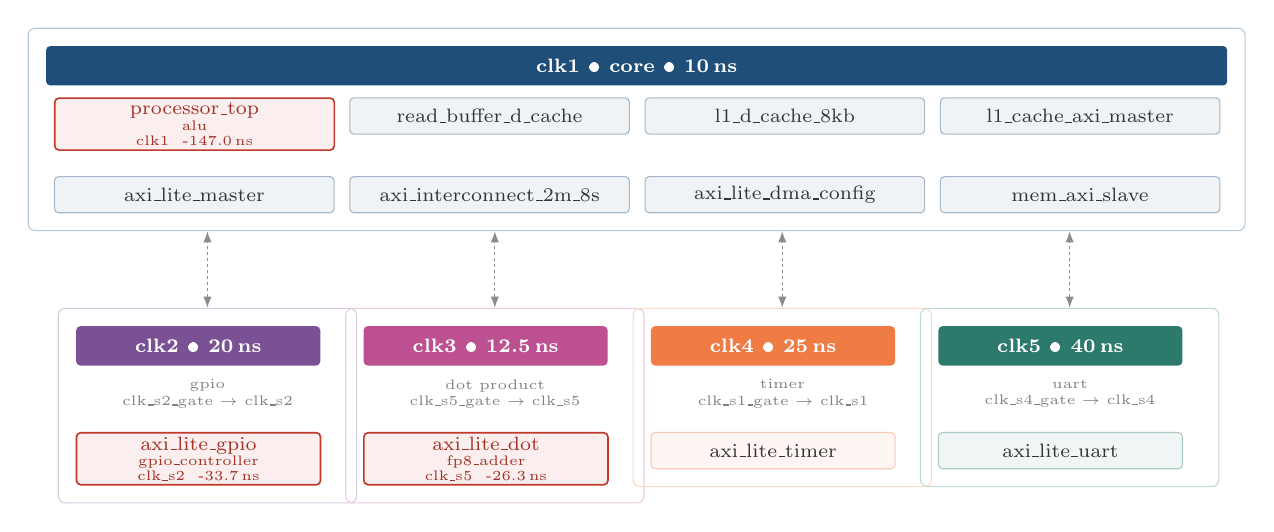
\begin{tikzpicture}[
    font=\scriptsize,
    blk/.style 2 args={rounded corners=1.5pt, draw=#1!40,
        fill=#1!7, text=black!80, minimum width=#2,
        minimum height=4.6mm, align=center, inner sep=1pt},
    hot/.style 2 args={rounded corners=1.5pt, draw=critical,
        line width=0.6pt, fill=critical!8, minimum width=#2,
        minimum height=6.6mm, align=center, inner sep=1pt,
        text=critical!85!black},
    hdr/.style={rounded corners=1.5pt, fill=#1, text=white,
        minimum height=5mm, align=center, inner sep=1pt},
    lane/.style={rounded corners=2.5pt, draw=#1!30, inner sep=2.2mm},
    chain/.style={font=\tiny, text=black!50, align=center},
    cdc/.style={{Latex[length=1.4mm]}-{Latex[length=1.4mm]},
        draw=black!45, dashed, dash pattern=on 1.1pt off 1.1pt,
        line width=0.45pt},
  ]
  \node[hdr=core, minimum width=150.0mm] (corehdr) at (0mm,0mm) {};
  \node[font=\scriptsize\bfseries, text=white] at (corehdr) {clk1 \textbullet\ core \textbullet\ 10\,ns};
  \node[hot={core}{35.5mm}, anchor=north west] (processor_top) at (-74.00mm,-4.00mm) {processor\_top\\[-2.5pt]{\tiny alu}\\[-2.5pt]{\tiny clk1\ \ -147.0\,ns}};
  \node[blk={core}{35.5mm}, anchor=north west] (read_buffer_d_cache) at (-36.50mm,-4.00mm) {read\_buffer\_d\_cache};
  \node[blk={core}{35.5mm}, anchor=north west] (l1_d_cache_8kb) at (1.00mm,-4.00mm) {l1\_d\_cache\_8kb};
  \node[blk={core}{35.5mm}, anchor=north west] (l1_cache_axi_master) at (38.50mm,-4.00mm) {l1\_cache\_axi\_master};
  \node[blk={core}{35.5mm}, anchor=north west] (axi_lite_master) at (-74.00mm,-14.00mm) {axi\_lite\_master};
  \node[blk={core}{35.5mm}, anchor=north west] (axi_interconnect_2m_8s) at (-36.50mm,-14.00mm) {axi\_interconnect\_2m\_8s};
  \node[blk={core}{35.5mm}, anchor=north west] (axi_lite_dma_config) at (1.00mm,-14.00mm) {axi\_lite\_dma\_config};
  \node[blk={core}{35.5mm}, anchor=north west] (mem_axi_slave) at (38.50mm,-14.00mm) {mem\_axi\_slave};
  \node[lane=core, fit=(corehdr)(processor_top)(read_buffer_d_cache)(l1_d_cache_8kb)(l1_cache_axi_master)(axi_lite_master)(axi_interconnect_2m_8s)(axi_lite_dma_config)(mem_axi_slave)] (corelane) {};
  \node[hdr=gpio, minimum width=31.0mm, anchor=north west] (h1) at (-71.25mm,-33.00mm) {};
  \node[font=\scriptsize\bfseries, text=white] at (h1) {clk2 \textbullet\ 20\,ns};
  \node[chain, anchor=north west, text width=31.0mm] (c1) at (-71.25mm,-38.60mm) {gpio\\clk\_s2\_gate $\rightarrow$ clk\_s2};
  \node[hot={gpio}{31.0mm}, anchor=north west] (axi_lite_gpio) at (-71.25mm,-46.50mm) {axi\_lite\_gpio\\[-2.5pt]{\tiny gpio\_controller}\\[-2.5pt]{\tiny clk\_s2\ \ -33.7\,ns}};
  \node[lane=gpio, fit=(h1)(c1)(axi_lite_gpio)] (lane1) {};
  \draw[cdc] (lane1.north) -- (lane1.north |- corelane.south);
  \node[hdr=dot, minimum width=31.0mm, anchor=north west] (h2) at (-34.75mm,-33.00mm) {};
  \node[font=\scriptsize\bfseries, text=white] at (h2) {clk3 \textbullet\ 12.5\,ns};
  \node[chain, anchor=north west, text width=31.0mm] (c2) at (-34.75mm,-38.60mm) {dot product\\clk\_s5\_gate $\rightarrow$ clk\_s5};
  \node[hot={dot}{31.0mm}, anchor=north west] (axi_lite_dot) at (-34.75mm,-46.50mm) {axi\_lite\_dot\\[-2.5pt]{\tiny fp8\_adder}\\[-2.5pt]{\tiny clk\_s5\ \ -26.3\,ns}};
  \node[lane=dot, fit=(h2)(c2)(axi_lite_dot)] (lane2) {};
  \draw[cdc] (lane2.north) -- (lane2.north |- corelane.south);
  \node[hdr=timer, minimum width=31.0mm, anchor=north west] (h3) at (1.75mm,-33.00mm) {};
  \node[font=\scriptsize\bfseries, text=white] at (h3) {clk4 \textbullet\ 25\,ns};
  \node[chain, anchor=north west, text width=31.0mm] (c3) at (1.75mm,-38.60mm) {timer\\clk\_s1\_gate $\rightarrow$ clk\_s1};
  \node[blk={timer}{31.0mm}, anchor=north west] (axi_lite_timer) at (1.75mm,-46.50mm) {axi\_lite\_timer};
  \node[lane=timer, fit=(h3)(c3)(axi_lite_timer)] (lane3) {};
  \draw[cdc] (lane3.north) -- (lane3.north |- corelane.south);
  \node[hdr=uart, minimum width=31.0mm, anchor=north west] (h4) at (38.25mm,-33.00mm) {};
  \node[font=\scriptsize\bfseries, text=white] at (h4) {clk5 \textbullet\ 40\,ns};
  \node[chain, anchor=north west, text width=31.0mm] (c4) at (38.25mm,-38.60mm) {uart\\clk\_s4\_gate $\rightarrow$ clk\_s4};
  \node[blk={uart}{31.0mm}, anchor=north west] (axi_lite_uart) at (38.25mm,-46.50mm) {axi\_lite\_uart};
  \node[lane=uart, fit=(h4)(c4)(axi_lite_uart)] (lane4) {};
  \draw[cdc] (lane4.north) -- (lane4.north |- corelane.south);
  \end{tikzpicture}
  \caption{The benchmark SoC as its SDC and RTL define it, generated from both rather than drawn by hand. Five mutually asynchronous masters, each peripheral domain built as master $\rightarrow$ gate $\rightarrow$ divider; every peripheral keeps its AXI-Lite side in the core domain and its functional side in its own, so each dashed line is a real clock-domain crossing. Outlined in red are the three blocks that own a violating path, each labelled with the module inside it that carries the delay, the clock it fails on and its baseline slack.}
  \label{fig:soc}
\end{figure}


\subsection{Why it is shaped this way}

A benchmark on which every path closes measures nothing, and one on which
nothing closes measures nothing either. This design is built to contain both,
and Figure~\ref{fig:soc} shows where.

\begin{itemize}
  \item \textbf{Five asynchronous masters.} They share no clock tree at
        all: the SDC declares them
        \texttt{-asynchronous} as five groups, so each domain closes or fails
        on its own. One global number cannot answer five
        independent closure questions, and this design is where that shows.
  \item \textbf{A gate and a divider on every master.} Each domain runs
        master $\rightarrow$ \texttt{clk\_gate} $\rightarrow$
        \texttt{clk\_div\_mux} $\rightarrow$ functional clock, giving divide
        by 1, 2, 4 or 8 under software control, constrained at divide-by-1
        (Section~\ref{sec:clocktree}).
  \item \textbf{Crossings that are real.} Every peripheral has its AXI-Lite
        side in the core domain and its functional side in its own, so each
        one is a genuine crossing rather than a decorative one.
  \item \textbf{Paths a transform can reach, and paths it cannot.} The
        slicer's three targets are outlined in Figure~\ref{fig:soc}. Two sit
        behind restructurable arithmetic. The third is a 32-step
        combinational restoring divider inside \texttt{alu}, at
        \baselinewns\,ns on the routed baseline, and no permitted transform
        reaches it without
        changing latency. It is in the benchmark on purpose.
\end{itemize}

\subsection{The clock tree}
\label{sec:clocktree}

Every clock in Table~\ref{tab:clocks} is declared, not inferred. The five
masters are created with \texttt{create\_clock}; everything below them is a
\texttt{create\_generated\_clock} that names its source, so the analyser walks
the gate and the divider as clock logic rather than treating their outputs as
unclocked nets and silently dropping the paths behind them. That distinction
is what makes the per-domain slack numbers in this report mean anything: a
domain whose functional clock is unrecognised reports no violations because it
reports no paths.

The divide ratio is software-controlled at 1, 2, 4 or 8, and the constraints
pin it at 1. That is the fastest the mux output can be, so it is the hardest
case; a design that closes at divide-by-1 closes at every other setting, and
constraining the slow settings instead would have made closure look easier
than it is.

% Generated by scripts/build_figures.py -- do not edit.
\begin{figure}[htbp]
  \centering
  \begin{adjustbox}{max width=\textwidth}
  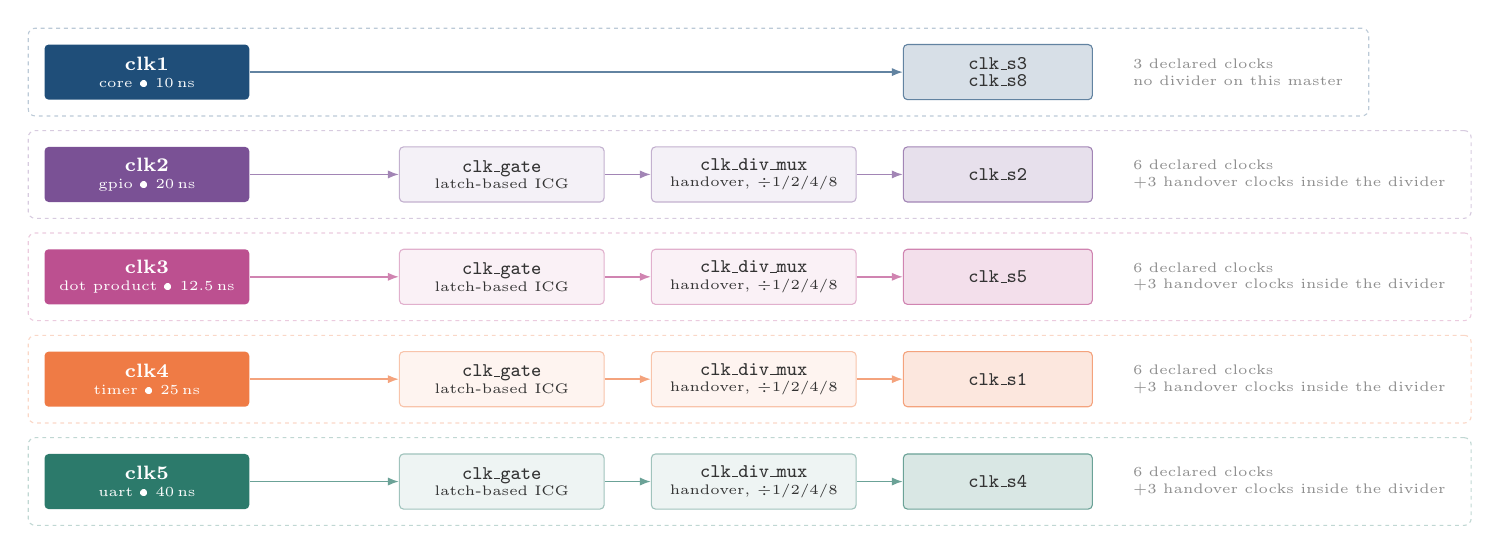
\begin{tikzpicture}[
    font=\scriptsize,
    master/.style={rounded corners=1.5pt, fill=#1, text=white,
        minimum width=26mm, minimum height=7mm, align=center,
        font=\scriptsize\bfseries, inner sep=1pt},
    cell/.style={rounded corners=1.5pt, draw=#1!45, fill=#1!8,
        minimum width=26mm, minimum height=7mm, align=center,
        inner sep=1pt, text=black!80},
    out/.style={rounded corners=1.5pt, draw=#1!70, fill=#1!18,
        minimum width=24mm, minimum height=7mm, align=center,
        inner sep=1pt, font=\scriptsize\bfseries, text=black!80},
    arr/.style={-{Latex[length=1.4mm]}, draw=#1!70, line width=0.5pt},
    grp/.style={rounded corners=2.5pt, draw=#1!30, dashed,
        dash pattern=on 1.4pt off 1.4pt, inner sep=2mm},
    tag/.style={font=\tiny, text=black!45, align=left},
  ]
  \node[master=core] (m0) at (0mm,0.0mm) {clk1\\[-2pt]{\tiny\mdseries core \textbullet\ 10\,ns}};
  \node[out=core, anchor=west] (o0) at (96mm,0.0mm) {\texttt{clk\_s3}\\[-2pt]\texttt{clk\_s8}};
  \draw[arr=core] (m0.east) -- (o0.west);
  \node[tag, anchor=west] (t0) at (124mm,0.0mm) {3 declared clocks\\no divider on this master};
  \node[grp=core, fit=(m0)(o0)(t0)] (grp0) {};
  \node[master=gpio] (m1) at (0mm,-13.0mm) {clk2\\[-2pt]{\tiny\mdseries gpio \textbullet\ 20\,ns}};
  \node[cell=gpio, anchor=west] (g1) at (32mm,-13.0mm) {\texttt{clk\_gate}\\[-2pt]{\tiny latch-based ICG}};
  \draw[arr=gpio] (m1.east) -- (g1.west);
  \node[cell=gpio, anchor=west] (d1) at (64mm,-13.0mm) {\texttt{clk\_div\_mux}\\[-2pt]{\tiny handover, $\div$1/2/4/8}};
  \draw[arr=gpio] (g1.east) -- (d1.west);
  \node[out=gpio, anchor=west] (o1) at (96mm,-13.0mm) {\texttt{clk\_s2}};
  \draw[arr=gpio] (d1.east) -- (o1.west);
  \node[tag, anchor=west] (t1) at (124mm,-13.0mm) {6 declared clocks\\+3 handover clocks inside the divider};
  \node[grp=gpio, fit=(m1)(g1)(d1)(o1)(t1)] (grp1) {};
  \node[master=dot] (m2) at (0mm,-26.0mm) {clk3\\[-2pt]{\tiny\mdseries dot product \textbullet\ 12.5\,ns}};
  \node[cell=dot, anchor=west] (g2) at (32mm,-26.0mm) {\texttt{clk\_gate}\\[-2pt]{\tiny latch-based ICG}};
  \draw[arr=dot] (m2.east) -- (g2.west);
  \node[cell=dot, anchor=west] (d2) at (64mm,-26.0mm) {\texttt{clk\_div\_mux}\\[-2pt]{\tiny handover, $\div$1/2/4/8}};
  \draw[arr=dot] (g2.east) -- (d2.west);
  \node[out=dot, anchor=west] (o2) at (96mm,-26.0mm) {\texttt{clk\_s5}};
  \draw[arr=dot] (d2.east) -- (o2.west);
  \node[tag, anchor=west] (t2) at (124mm,-26.0mm) {6 declared clocks\\+3 handover clocks inside the divider};
  \node[grp=dot, fit=(m2)(g2)(d2)(o2)(t2)] (grp2) {};
  \node[master=timer] (m3) at (0mm,-39.0mm) {clk4\\[-2pt]{\tiny\mdseries timer \textbullet\ 25\,ns}};
  \node[cell=timer, anchor=west] (g3) at (32mm,-39.0mm) {\texttt{clk\_gate}\\[-2pt]{\tiny latch-based ICG}};
  \draw[arr=timer] (m3.east) -- (g3.west);
  \node[cell=timer, anchor=west] (d3) at (64mm,-39.0mm) {\texttt{clk\_div\_mux}\\[-2pt]{\tiny handover, $\div$1/2/4/8}};
  \draw[arr=timer] (g3.east) -- (d3.west);
  \node[out=timer, anchor=west] (o3) at (96mm,-39.0mm) {\texttt{clk\_s1}};
  \draw[arr=timer] (d3.east) -- (o3.west);
  \node[tag, anchor=west] (t3) at (124mm,-39.0mm) {6 declared clocks\\+3 handover clocks inside the divider};
  \node[grp=timer, fit=(m3)(g3)(d3)(o3)(t3)] (grp3) {};
  \node[master=uart] (m4) at (0mm,-52.0mm) {clk5\\[-2pt]{\tiny\mdseries uart \textbullet\ 40\,ns}};
  \node[cell=uart, anchor=west] (g4) at (32mm,-52.0mm) {\texttt{clk\_gate}\\[-2pt]{\tiny latch-based ICG}};
  \draw[arr=uart] (m4.east) -- (g4.west);
  \node[cell=uart, anchor=west] (d4) at (64mm,-52.0mm) {\texttt{clk\_div\_mux}\\[-2pt]{\tiny handover, $\div$1/2/4/8}};
  \draw[arr=uart] (g4.east) -- (d4.west);
  \node[out=uart, anchor=west] (o4) at (96mm,-52.0mm) {\texttt{clk\_s4}};
  \draw[arr=uart] (d4.east) -- (o4.west);
  \node[tag, anchor=west] (t4) at (124mm,-52.0mm) {6 declared clocks\\+3 handover clocks inside the divider};
  \node[grp=uart, fit=(m4)(g4)(d4)(o4)(t4)] (grp4) {};
  \end{tikzpicture}
  \end{adjustbox}
  \caption{The five clock domains, one chain each, read out of \texttt{nebula.sdc}. Each dashed box is one \texttt{-asynchronous} group: nothing inside it is timed against anything inside another. The core master drives its generated clocks directly; the four peripheral masters each run through a latch-based clock gate and a handover divider, whose internal clocks are declared and joined to the same group rather than left for the analyser to guess at.}
  \label{fig:clocktree}
\end{figure}


\begin{table}[htbp]
  \centering
  \footnotesize
  \caption{Every clock the design declares. The five masters are mutually asynchronous; each generated clock names the source it is derived from, so the analyser follows the gate and divider chain instead of treating their outputs as unclocked nets.}
  \label{tab:clocks}
  \begin{adjustbox}{max width=\textwidth}
  \begin{tabular}{llrrll}
    \toprule
    \textbf{Clock} & \textbf{Kind} & \textbf{Source} & \textbf{Period (ns)} & \textbf{Role} & \textbf{Baseline WNS} \\
    \midrule
    \texttt{clk1} & master & -- & 10 & core        100 MHz & -126.6293 \\
    \texttt{clk2} & master & -- & 20 & gpio         50 MHz & {\footnotesize no endpoints} \\
    \texttt{clk3} & master & -- & 12.5 & dot product  80 MHz & {\footnotesize no endpoints} \\
    \texttt{clk4} & master & -- & 25 & timer        40 MHz & {\footnotesize no endpoints} \\
    \texttt{clk5} & master & -- & 40 & uart         25 MHz & {\footnotesize no endpoints} \\
    \texttt{clk\_s1\_gate} & generated & \texttt{clk4} & 25.0 & divide by 1 & 23.1259 \\
    \texttt{clk\_s2\_gate} & generated & \texttt{clk2} & 20.0 & divide by 1 & 17.9242 \\
    \texttt{clk\_s5\_gate} & generated & \texttt{clk3} & 12.5 & divide by 1 & 10.5934 \\
    \texttt{clk\_s4\_gate} & generated & \texttt{clk5} & 40.0 & divide by 1 & 37.8683 \\
    \texttt{clk\_s3} & generated & \texttt{clk1} & 10.0 & divide by 1 & -0.1019 \\
    \texttt{clk\_s8} & generated & \texttt{clk1} & 10.0 & divide by 1 & -3.3171 \\
    \texttt{clk\_s1} & generated & \texttt{clk\_s1\_gate} & 25.0 & divide by 1 & 16.9266 \\
    \texttt{clk\_s2} & generated & \texttt{clk\_s2\_gate} & 20.0 & divide by 1 & -27.8000 \\
    \texttt{clk\_s5} & generated & \texttt{clk\_s5\_gate} & 12.5 & divide by 1 & -29.3740 \\
    \texttt{clk\_s4} & generated & \texttt{clk\_s4\_gate} & 40.0 & divide by 1 & 0.1477 \\
    \bottomrule
  \end{tabular}
  \end{adjustbox}
  \par\smallskip\footnotesize\raggedright `no endpoints' is a domain in which nothing is clocked directly: every flop behind those four masters sits on the generated clock after the gate and divider, so the master itself owns no constrained path. Generated clocks are declared divide-by-1 because that is the fastest the divider mux can run, and a design that closes there closes at every other setting.
\end{table}


\subsection{The clock structures, and the two bugs that were in them}

The five domains are clean as \emph{constraints}: every clock is declared,
every generated clock names its source, and the five masters are grouped
asynchronous, so timing is analysed correctly across the whole tree. The RTL
that builds them is a different question, and the first version of this
benchmark got it wrong twice. \texttt{clk\_gate} was a bare
\texttt{clk\_in \& clk\_en}: an enable change while the clock is high chops
the pulse. \texttt{clk\_div\_mux} selected combinationally among four clocks:
a select change mid-pulse truncates it. Both are the textbook glitch, and both
survived synthesis, timing analysis and equivalence checking without a
complaint from any of them, because none of those three tools is looking.
Equivalence checking compares functions and a runt pulse is not a function;
static timing analysis is \emph{told} the net is a clock and believes it.

That is why this project has a third structural check,
\texttt{clockcheck.py}, and why the audit it produces
(Table~\ref{tab:clockrisk}) is in the report. It found both structures, and
both were then rewritten rather than merely disclosed: the gate into a
latch-based integrated clock gate, whose enable can only change while the
clock is already low, and the divider select into a handover mux in which
each branch is gated by an enable registered on that branch's own falling
edge and may assert only once every other branch has released. The audit now
returns \clockverdict{} over \clockfindings{} clock structures, with
\clockglitchy{} glitch findings.

An audit passing is not on its own evidence, because the auditor is a shape
recogniser and the shapes are ones we wrote down. The evidence is a
simulation that measures pulse widths on both outputs while switching the
divide ratio \SI{2}{\nano\second} after a rising edge, while the
selected clock is high and a combinational mux would cut the pulse, and by
toggling the gate enable at odd phases. The fixed structures produce \runtsfixed{} runt
pulses. The same testbench on the original structures produces
\runtscontrol{}, which is the number that matters: a runt check that passes
on a design known to produce runts is measuring nothing.

The cost is paid in the constraints, not hidden from them. The handover flops
are clocked by the divider's own counter bits, so those twelve internal nets
are now real clocks with real registers behind them; each is declared as a
generated clock of its domain and joins that domain's asynchronous group. Left
undeclared they would have been unclocked registers, and an unclocked register
raises no warning in a timing report. It is a path that quietly stops being
analysed.

\begin{figure}[htbp]
  \centering
  \begin{adjustbox}{max width=\textwidth}
  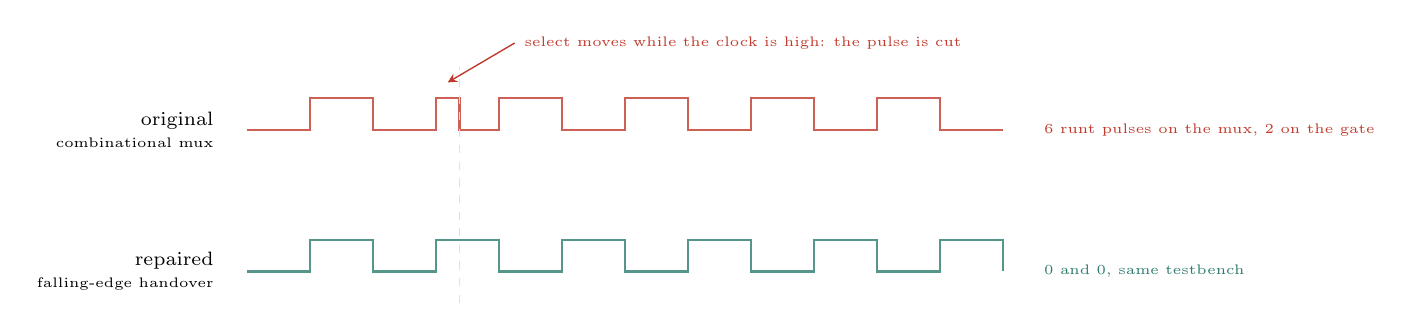
\begin{tikzpicture}[font=\scriptsize]
  \node[anchor=east, align=right, font=\scriptsize] at (-3mm,4mm) {original\\{\tiny combinational mux}};
  \draw[critical!80, line width=0.8pt] (0mm,4mm+0mm) -- (8mm,4mm+0mm) -- (8mm,4mm+4mm) -- (8mm,4mm+4mm) -- (16mm,4mm+4mm) -- (16mm,4mm+0mm) -- (16mm,4mm+0mm) -- (24mm,4mm+0mm) -- (24mm,4mm+4mm) -- (24mm,4mm+4mm) -- (27mm,4mm+4mm) -- (27mm,4mm+0mm) -- (27mm,4mm+0mm) -- (32mm,4mm+0mm) -- (32mm,4mm+4mm) -- (32mm,4mm+4mm) -- (40mm,4mm+4mm) -- (40mm,4mm+0mm) -- (40mm,4mm+0mm) -- (48mm,4mm+0mm) -- (48mm,4mm+4mm) -- (48mm,4mm+4mm) -- (56mm,4mm+4mm) -- (56mm,4mm+0mm) -- (56mm,4mm+0mm) -- (64mm,4mm+0mm) -- (64mm,4mm+4mm) -- (64mm,4mm+4mm) -- (72mm,4mm+4mm) -- (72mm,4mm+0mm) -- (72mm,4mm+0mm) -- (80mm,4mm+0mm) -- (80mm,4mm+4mm) -- (80mm,4mm+4mm) -- (88mm,4mm+4mm) -- (88mm,4mm+0mm) -- (88mm,4mm+0mm) -- (96mm,4mm+0mm) -- (96mm,4mm+0mm) -- (96mm,4mm+0mm);
  \draw[critical, <-, >=stealth, line width=0.5pt] (25.5mm,10mm) -- (34mm,15mm) node[right, font=\tiny, text=critical] {select moves while the clock is high: the pulse is cut};
  \node[anchor=east, align=right, font=\scriptsize] at (-3mm,-14mm) {repaired\\{\tiny falling-edge handover}};
  \draw[accepted!80, line width=0.8pt] (0mm,-14mm+0mm) -- (8mm,-14mm+0mm) -- (8mm,-14mm+4mm) -- (8mm,-14mm+4mm) -- (16mm,-14mm+4mm) -- (16mm,-14mm+0mm) -- (16mm,-14mm+0mm) -- (24mm,-14mm+0mm) -- (24mm,-14mm+4mm) -- (24mm,-14mm+4mm) -- (32mm,-14mm+4mm) -- (32mm,-14mm+0mm) -- (32mm,-14mm+0mm) -- (40mm,-14mm+0mm) -- (40mm,-14mm+4mm) -- (40mm,-14mm+4mm) -- (48mm,-14mm+4mm) -- (48mm,-14mm+0mm) -- (48mm,-14mm+0mm) -- (56mm,-14mm+0mm) -- (56mm,-14mm+4mm) -- (56mm,-14mm+4mm) -- (64mm,-14mm+4mm) -- (64mm,-14mm+0mm) -- (64mm,-14mm+0mm) -- (72mm,-14mm+0mm) -- (72mm,-14mm+4mm) -- (72mm,-14mm+4mm) -- (80mm,-14mm+4mm) -- (80mm,-14mm+0mm) -- (80mm,-14mm+0mm) -- (88mm,-14mm+0mm) -- (88mm,-14mm+4mm) -- (88mm,-14mm+4mm) -- (96mm,-14mm+4mm) -- (96mm,-14mm+0mm) -- (96mm,-14mm+0mm);
  \draw[rule!60, dashed, line width=0.4pt] (27mm,-18mm) -- (27mm,12mm);
  \node[anchor=west, font=\tiny, text=critical] at (100mm,4mm) {6 runt pulses on the mux, 2 on the gate};
  \node[anchor=west, font=\tiny, text=accepted] at (100mm,-14mm) {0 and 0, same testbench};
  \end{tikzpicture}
  \end{adjustbox}
  \caption{The clock-divider mux before and after the repair, with the pulse widths a simulation measured on each. The traces are schematic; the counts beside them are the testbench's, and the upper row is the original RTL run through the identical stimulus.}
  \label{fig:runt}
  \par\smallskip\footnotesize\raggedright A runt check that passes on a design known to produce runts measures nothing, so the repaired structure is reported against a control that fails rather than on its own.
\end{figure}


\begin{table}[htbp]
  \centering
  \footnotesize
  \caption{The clock-structure audit of the benchmark. Both structures started glitchy -- a bare AND clock gate and a combinational clock mux -- and both were rewritten: the gate into a latch-based ICG, the divider select into a handover mux whose branches are enabled by flops on their own clock. Simulation agrees with the audit: 0 runt pulses on the fixed structures against 8 on the originals under the same stimulus, which switches the divider select while the selected clock is high.}
  \label{tab:clockrisk}
  \begin{adjustbox}{max width=\textwidth}
  \begin{tabular}{lllp{62mm}}
    \toprule
    \textbf{Module} & \textbf{Net} & \textbf{Verdict} & \textbf{What the auditor found} \\
    \midrule
    \texttt{clk\_div\_mux} & \texttt{clk\_out} & \texttt{SAFE\_MUX} & clk\_out hands over between clk, clk\_div2, clk\_div4, clk\_div8: each branch is gated by an enable registered on that branch's own falling edge and may only assert once every other branch has released, so the output is whole pulses of one source \\
    \texttt{clk\_gate} & \texttt{clk\_out} & \texttt{SAFE\_ICG} & clk\_out = clk\_in \& latched enable (en\_latch) \\
    \bottomrule
  \end{tabular}
  \end{adjustbox}
\end{table}


\subsection{Scale}

The competition asks for roughly \num{50000} standard cells, and
Table~\ref{tab:scale} reports what the frozen input actually is after a
complete place-and-route run rather than what the RTL was intended to be.
Cell count is taken from the routed database, not from a synthesis estimate,
because the two differ by more than the tolerance any claim here would need.

\begin{table}[htbp]
  \centering
  \footnotesize
  \caption{The benchmark at the scale the competition asks for, measured on the routed baseline rather than estimated from the RTL.}
  \label{tab:scale}
  \begin{adjustbox}{max width=\textwidth}
  \begin{tabular}{lr}
    \toprule
    \textbf{} & \textbf{Frozen input, post-route} \\
    \midrule
    RTL modules & 59 \\
    RTL lines & 12\,015 \\
    Master clock domains & 5, mutually asynchronous \\
    Clocks declared & 15 \\
    Placed instances & 488\,118 \\
    Nets & 143\,367 \\
    Die area & 1914043\,\si{\um\squared} \\
    Routed wirelength & 7409236\,\si{\um} \\
    Utilisation & 54.0\,\% \\
    PDK & sky130hd, via OpenROAD-flow-scripts \\
    \bottomrule
  \end{tabular}
  \end{adjustbox}
\end{table}


% =====================================================================
\section{Baselines}

Three different things are called a baseline in this report, and conflating
them is the easiest way to overstate a result, so they are named separately.

\subsection{The frozen input}

The RTL in \texttt{bench/rtl\_v2} is never edited by hand. Every number
labelled \emph{baseline} is
measured on that tree taken through the same synthesis, placement and routing
as every variant, with the same PDK, the same constraints and the same flow
settings. A variant is compared only against that run, never against another
variant, which is what makes the deltas addable into one table.

\subsection{The un-gated model}

The interesting baseline is not ``no LLM''. It is ``the same LLM with the gates
switched off'', because that is what most published RTL-repair loops are. This report does not have to simulate it: the gates recorded what they
caught, and every row in Table~\ref{tab:g1b} is an edit an un-gated loop would
have shipped. Those rewrites are formally equivalent to the module they
replace, under a complete proof, and still wrong in the design, because the
parent that instantiates them no longer meets its contract. A loop whose
acceptance test is ``does it still simulate'' or ``did the model say it was
safe'' accepts all of them.

\subsection{The published systems}
\label{sec:related}

ViTAD reports 73.68\% repair success against 54.38\% for a plain-LLM baseline,
and is the closest published architecture to this one: parse the RTL and the
timing report, build a dependency graph, have the model infer a root cause,
generate a targeted fix. AutoChip closes the same loop with compiler and
simulation feedback. SymRTLO adds retrieval and a symbolic FSM pass.

None of them gates on formal equivalence before accepting. That is the
difference this report is built around, and it is why the numbers here are not
directly comparable to a repair-rate percentage: a system that accepts on
simulation and a system that accepts on proof are not measuring the same
event. What can be compared is what each system would have done with the
rewrites in Table~\ref{tab:g1b}, and the answer is that they would have taken
them.

% =====================================================================
\section{Deliverable 1 --- RTL timing analysis framework}
\label{sec:d1}

OpenSTA is driven from TCL and returns ranked critical paths as structured
JSON, which is what the model consumes as context. Paths are sliced from the
post-synthesis database rather than the post-resizer netlist: the resizer had
already absorbed two of the three domains' violations into buffering, so a
slicer reading that netlist reported closure the RTL had not achieved.

Each path is annotated with the module that owns it, that module's parents, and
whether an RTL lever exists at all. Targets with no lever are still reported and
are not sent to a model, which is where most of the call budget was being spent
before the annotation existed.

% =====================================================================
\section{Deliverable 2 --- GenAI-based RTL optimisation engine}
\label{sec:d2}

The loop is \texttt{run\_sta} $\rightarrow$ \texttt{propose} $\rightarrow$
\texttt{gate} $\rightarrow$ \texttt{accept or feed back}. What distinguishes it
from the published systems we compared against is that rejection is
mechanical and specific: the model is told which gate rejected it and what the
gate found, and the next attempt answers that.

\subsection{The gates}
\label{sec:gates}

\begin{itemize}
  \item \textbf{G1 --- module equivalence.} The rewritten module against the
        frozen one. Combinational modules are proved complete in a single
        miter cycle; a feed-forward pipeline insertion is complete at
        latency${}+2$; everything else is bounded and reported as bounded.
  \item \textbf{G1b --- parent contract.} The parent instantiating the rewritten
        module, proved at \emph{its} boundary. A module may be equivalent to its
        original and still break the parent, and this is the gate that catches
        it.
  \item \textbf{G1c --- clock structure at the boundary.}
  \item \textbf{G2 / G2c --- clock-domain crossings, and a clock-structure
        regression against the baseline.} A structure the baseline already
        has is allowed; a newly created glitchy one is not.
  \item \textbf{G3 --- place and route.} Run once over the accumulated set.
\end{itemize}

% Generated by scripts/build_figures.py -- do not edit.
\begin{figure}[htbp]
  \centering
  \begin{adjustbox}{max width=\textwidth}
  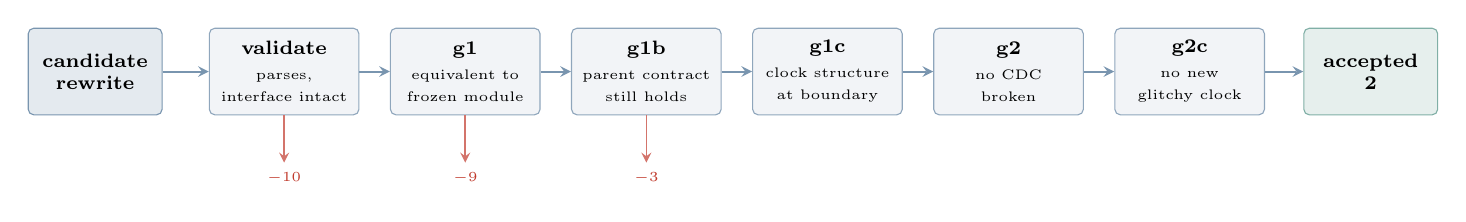
\begin{tikzpicture}[
    font=\scriptsize,
    gate/.style={rounded corners=2pt, draw=accent!50,
                 fill=accent!6, minimum width=19mm,
                 minimum height=11mm, align=center},
    term/.style={rounded corners=2pt, draw=#1!60, fill=#1!12,
                 minimum width=17mm, minimum height=11mm,
                 align=center, font=\scriptsize\bfseries},
    flow/.style={->, >=stealth, draw=accent!60, line width=0.7pt},
    drop/.style={->, >=stealth, draw=critical!70, line width=0.6pt},
  ]
  \node[term=accent] (in) at (0mm,0) {candidate\\rewrite};
  \node[gate] (validate) at (24.0mm, 0) {\textbf{validate}\\[1pt]{\tiny parses,}\\{\tiny interface intact}};
  \draw[flow] (in) -- (validate);
  \draw[drop] (validate.south) -- ++(0,-6mm) node[below, font=\tiny, text=critical] {$-$10};
  \node[gate] (g1) at (47.0mm, 0) {\textbf{g1}\\[1pt]{\tiny equivalent to}\\{\tiny frozen module}};
  \draw[flow] (validate) -- (g1);
  \draw[drop] (g1.south) -- ++(0,-6mm) node[below, font=\tiny, text=critical] {$-$9};
  \node[gate] (g1b) at (70.0mm, 0) {\textbf{g1b}\\[1pt]{\tiny parent contract}\\{\tiny still holds}};
  \draw[flow] (g1) -- (g1b);
  \draw[drop] (g1b.south) -- ++(0,-6mm) node[below, font=\tiny, text=critical] {$-$3};
  \node[gate] (g1c) at (93.0mm, 0) {\textbf{g1c}\\[1pt]{\tiny clock structure}\\{\tiny at boundary}};
  \draw[flow] (g1b) -- (g1c);
  \node[gate] (g2) at (116.0mm, 0) {\textbf{g2}\\[1pt]{\tiny no CDC}\\{\tiny broken}};
  \draw[flow] (g1c) -- (g2);
  \node[gate] (g2c) at (139.0mm, 0) {\textbf{g2c}\\[1pt]{\tiny no new}\\{\tiny glitchy clock}};
  \draw[flow] (g2) -- (g2c);
  \node[term=accepted] (ok) at (162.0mm, 0) {accepted\\2};
  \draw[flow] (g2c) -- (ok);
  \end{tikzpicture}
  \end{adjustbox}
  \caption{Every gate a rewrite must pass, with the number of candidates each one rejected across all four models. A gate rejects on its own evidence and reports what it found; the model's next attempt answers that, rather than being asked the same question again.}
  \label{fig:gates}
\end{figure}


A bounded proof limits only the right to declare equivalence. A counterexample
at step 0 or 1 is conclusive regardless of the bound, and rejections on that
basis are final.

\subsection{Multi-module edits}
\label{sec:multimodule}

A latency change is not a local edit: every parent has to learn to wait. The
harness accepts one proposal that rewrites the target and, through a
\texttt{submodules} field, every parent that must change with it, and proves
the set together. Without that channel the only legal edits are
latency-preserving ones, which rules out the transform that deep combinational
paths actually need.

\subsection{Scope is taken from the tree, not from the proposal}
\label{sec:scope}

A proposal names what it claims to edit. That claim is not evidence. Asked
about one module, a model re-sent an edit to a different module it had already
had accepted and left the named one byte-identical to the frozen input; every
gate passed, because proving an unchanged module against itself is trivially
true. The accepted set is therefore derived from what actually differs from the
working tree, and a proposal that differs nowhere is recorded as a no-op rather
than as a closed path.

% =====================================================================
\section{Deliverable 3 --- Critical path and timing violation analysis}
\label{sec:d3}

\begin{table}[htbp]
  \centering
  \footnotesize
  \caption{Where candidates died, summed over all four models. Each row is a rewrite that looked reasonable enough to reach that gate.}
  \label{tab:funnel}
  \begin{adjustbox}{max width=\textwidth}
  \begin{tabular}{llr}
    \toprule
    \textbf{Why the candidate was rejected} & \textbf{Gate} & \textbf{Count} \\
    \midrule
    reply unusable (truncated or unparseable) & \texttt{propose} & 21 \\
    did not parse as Verilog, or changed the interface & \texttt{validate} & 10 \\
    not equivalent to the frozen module & \texttt{g1} & 9 \\
    equivalent, but broke the parent's timing contract & \texttt{g1b} & 3 \\
    API call failed or was refused & \texttt{backend} & 1 \\
    \textbf{accepted} & \texttt{accepted} & \textbf{2} \\
    \bottomrule
  \end{tabular}
  \end{adjustbox}
  \par\smallskip\footnotesize\raggedright 46 candidates in total. The two rows below \texttt{g1} are the ones an equivalence-only flow would have shipped: they are formally equivalent to the frozen module and still wrong.
\end{table}


Table~\ref{tab:funnel} gives the full funnel. Most candidates are rejected
before any prover runs, and the largest single loss is not a model failure: it
is replies that exhausted their token budget inside reasoning and returned no
text. That is a harness defect, it is disclosed in
Table~\ref{tab:bakeoff} per arm, and it is corrected in the runs that followed.

The funnel counts the four bake-off arms only, and its accepted row is
therefore two, not \numaccepted. The third accepted edit is the same
\texttt{fp8\_adder} transform re-proposed in the re-run made after the harness
defect above was fixed; it is counted in \numaccepted{} and in
Table~\ref{tab:accepts}, which name the run each edit came from, and it is
deliberately not folded back into a funnel built from the four arms that ran
under the defective harness.

% =====================================================================
\section{Deliverable 4 --- Optimised RTL implementation}
\label{sec:d4}

\begin{table}[htbp]
  \centering
  \footnotesize
  \caption{Every edit the gate accepted, with the proof that admitted it. A complete proof settles equivalence for all inputs and all time; a bounded one limits only the right to declare equivalence, never the right to reject on a counterexample.}
  \label{tab:accepts}
  \begin{adjustbox}{max width=\textwidth}
  \begin{tabular}{llrllrrl}
    \toprule
    \textbf{Module} & \textbf{Transform} & \textbf{$\Delta$latency} & \textbf{G1 verdict} & \textbf{Proof} & \textbf{Complete} & \textbf{Solver (s)} & \textbf{Run} \\
    \midrule
    \texttt{fp8\_adder} & logic\_restructure & 0 & EQUIVALENT & combinational & \checkmark & 0.5 & \texttt{bakeoff\_v2\_sonnet\_fixed} \\
    \texttt{fp8\_adder} & logic\_restructure & 0 & EQUIVALENT & combinational & \checkmark & 0.3 & \texttt{anthropic\_sonnet-direct} \\
    \texttt{fp8\_adder} & logic\_restructure & 0 & EQUIVALENT & combinational & \checkmark & 0.4 & \texttt{openrouter\_nemotron-ultra} \\
    \bottomrule
  \end{tabular}
  \end{adjustbox}
  \par\smallskip\footnotesize\raggedright The module column lists what the run actually rewrote, derived from the working tree rather than from the proposal's own claim about its scope.
\end{table}


\begin{table}[htbp]
  \centering
  \footnotesize
  \caption{Rewrites that a formal equivalence check passed and the flow still rejected. These are the cases an EQY-only gate ships.}
  \label{tab:g1b}
  \begin{adjustbox}{max width=\textwidth}
  \begin{tabular}{llllll}
    \toprule
    \textbf{Module} & \textbf{Model} & \textbf{G1 verdict} & \textbf{Proof} & \textbf{Killed by} & \textbf{What the gate found} \\
    \midrule
    \texttt{fp4\_dot\_unit} & claude-sonnet-5 & EQUIVALENT & feed-forward & \texttt{g1b} & CONTRACT\_BROKEN at \texttt{axi\_lite\_dot} \\
    \texttt{fp4\_dot\_unit} & claude-opus-5 & EQUIVALENT & feed-forward & \texttt{g1b} & CONTRACT\_BROKEN at \texttt{axi\_lite\_dot} \\
    \texttt{fp4\_dot\_unit} & free & EQUIVALENT & feed-forward & \texttt{g1b} & CONTRACT\_BROKEN at \texttt{axi\_lite\_dot} \\
    \bottomrule
  \end{tabular}
  \end{adjustbox}
  \par\smallskip\footnotesize\raggedright Each of these is equivalent to the frozen module at its own boundary and still wrong in the design: equivalence is a statement about a function, and a pipeline stage is not only a function. That three independently developed models produce the same defect is the argument for checking it rather than reviewing for it.
\end{table}


Table~\ref{tab:g1b} is the result we would lead with if only one table
survived. Each row is a rewrite that a formal equivalence check passed with a complete
proof, not a bounded one, and that the flow rejected anyway,
because the module's parent no longer met its contract. Three independently
developed models produced the same class of defect, which is the argument for
gating it mechanically rather than trusting review to catch it.

% =====================================================================
\section{Deliverable 5 --- Timing, frequency and PPA comparison}
\label{sec:d5}

\begin{table}[htbp]
  \centering
  \footnotesize
  \caption{Post-route PPA, frozen input against each formally verified variant. Every variant is routed from the frozen RTL with only gate-accepted edits applied, and every figure is read from the same flow stage.}
  \label{tab:ppa}
  \begin{adjustbox}{max width=\textwidth}
  \begin{tabular}{lrrr}
    \toprule
    \textbf{Metric} & \textbf{Baseline} & \textbf{sonnet} & \textbf{nemotron-ultra} \\
    \midrule
    Setup WNS (ns) & -126.6293 & -124.1160 \tiny(+2.5133) & -130.0722 \tiny(-3.4429) \\
    Setup TNS (ns) & -97704.1 & -94156.3 \tiny(+3547.8) & -97854.0 \tiny(-149.9) \\
    Hold WNS (ns) & -0.0820 & -0.0583 & -0.1233 \\
    Area (\si{\um\squared}) & 1914043 & 1913142 & 1905391 \\
    Instances & 488118 & 488607 & 489340 \\
    Nets & 143367 & 143398 & 142790 \\
    Wirelength (\si{\um}) & 7409236 & 7382892 & 7376890 \\
    Utilisation (\%) & 54.0 & 54.0 & 54.0 \\
    DRC violations & 0 & 0 & 0 \\
    \bottomrule
  \end{tabular}
  \end{adjustbox}
  \par\smallskip\footnotesize\raggedright Bracketed figures are the delta against the baseline. Global WNS is set by a single unclosed path and is not a summary of the design; see Table~\ref{tab:fmax}.
\end{table}


\subsection{Why the global number is not the result}

Global WNS on this design is set by one path: a 32-step combinational restoring
divider, at \baselinewns\,ns. That path did not close, it is reported as not
closed, and it moves under placement variance by more than any edit moved it.
Quoting it as the headline would be reporting router noise.

\begin{table}[htbp]
  \centering
  \footnotesize
  \caption{Per-domain setup WNS and the frequency change it implies. The benchmark has five asynchronous masters and therefore five closure questions; collapsing them into one global number hides every result the run did produce.}
  \label{tab:fmax}
  \begin{adjustbox}{max width=\textwidth}
  \begin{tabular}{lrrrrrr}
    \toprule
    \textbf{Clock} & \textbf{Period (ns)} & \textbf{Base WNS} & \textbf{sonnet $\Delta$WNS} & \textbf{$\Delta F_{\max}$} & \textbf{nemotron-ultra $\Delta$WNS} & \textbf{$\Delta F_{\max}$} \\
    \midrule
    clk1 & 10.0 & -126.6293 & +2.5133 & +0.14 & -3.4429 & -0.18 \\
    clk\_s1 & 25.0 & 16.9266 & -0.2288 & -3.41 & -0.1127 & -1.71 \\
    clk\_s1\_gate & 25.0 & 23.1259 & -0.0174 & \emph{n/q} & +0.6316 & \emph{n/q} \\
    clk\_s2 & 20.0 & -27.8000 & +1.6039 & +0.73 & +1.6084 & +0.73 \\
    clk\_s2\_gate & 20.0 & 17.9242 & -0.1017 & \emph{n/q} & +0.3305 & \emph{n/q} \\
    clk\_s3 & 10.0 & -0.1019 & -0.0622 & -0.61 & -0.0510 & -0.50 \\
    clk\_s4 & 40.0 & 0.1477 & -0.5585 & -0.35 & +0.0213 & +0.01 \\
    clk\_s4\_gate & 40.0 & 37.8683 & -0.0551 & \emph{n/q} & +0.3229 & \emph{n/q} \\
    clk\_s5 & 12.5 & -29.3740 & -0.1006 & -0.06 & -0.1175 & -0.07 \\
    clk\_s5\_gate & 12.5 & 10.5934 & +0.4531 & \emph{n/q} & +0.1294 & \emph{n/q} \\
    clk\_s8 & 10.0 & -3.3171 & +1.1740 & +7.26 & +1.3806 & +8.69 \\
    \bottomrule
  \end{tabular}
  \end{adjustbox}
  \par\smallskip\footnotesize\raggedright $F_{\max}=1/(\text{period}-\text{WNS})$, per domain, holding everything else fixed; it is not the chip frequency, which the slowest domain still governs. \emph{n/q} marks a domain whose slack is nearly a full period: the reciprocal is ill-conditioned there and a hundredth of a nanosecond of placement variance moves it by hundreds of MHz, so the slack delta is reported and the frequency derived from it is withheld.
\end{table}


\begin{figure}[htbp]
  \centering
  \begin{adjustbox}{max width=\textwidth}
  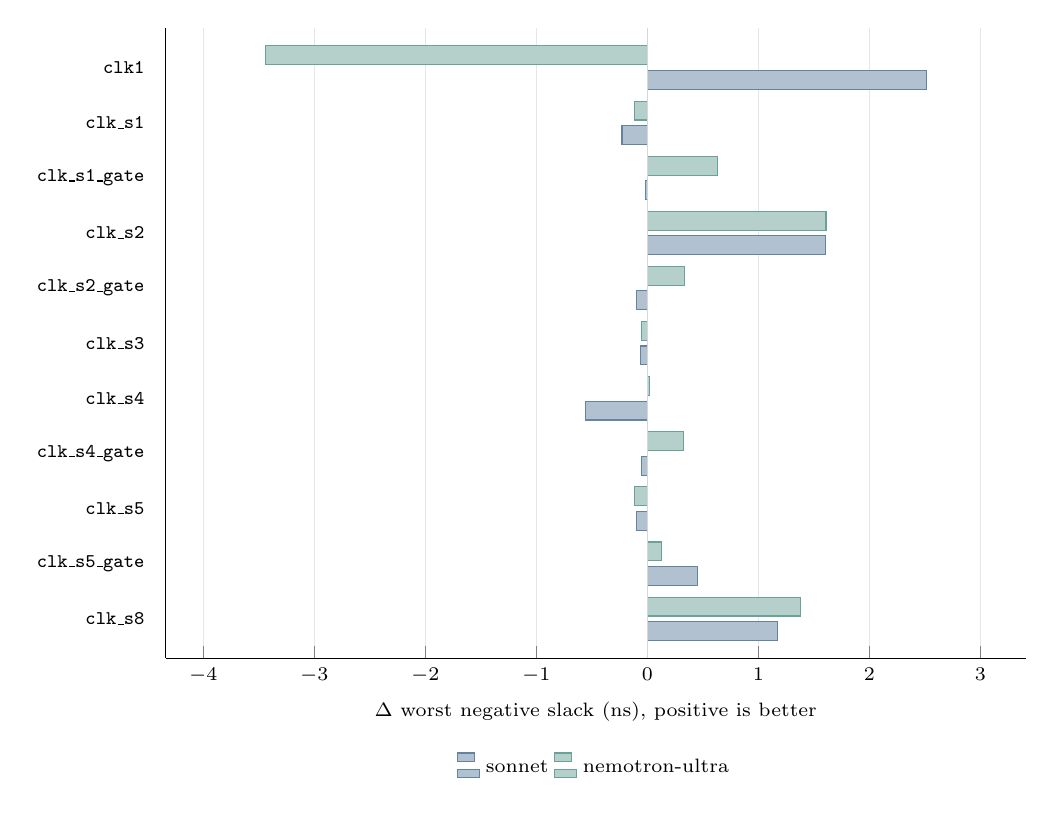
\begin{tikzpicture}
  \begin{axis}[
    xbar, width=125mm, height=91mm,
    bar width=2.4mm, y=7mm, font=\scriptsize,
    xlabel={$\Delta$ worst negative slack (ns), positive is better},
    ytick={0,1,2,3,4,5,6,7,8,9,10}, yticklabels={\texttt{clk1},\texttt{clk\_s1},\texttt{clk\_s1\_gate},\texttt{clk\_s2},\texttt{clk\_s2\_gate},\texttt{clk\_s3},\texttt{clk\_s4},\texttt{clk\_s4\_gate},\texttt{clk\_s5},\texttt{clk\_s5\_gate},\texttt{clk\_s8}},
    ytick style={draw=none}, y dir=reverse,
    axis x line*=bottom, axis y line*=left,
    xmajorgrids, grid style={rule!50, very thin},
    enlarge y limits={abs=5mm}, enlarge x limits=0.15,
    legend style={at={(0.5,-0.14)}, anchor=north, draw=none,
                  legend columns=-1, font=\scriptsize},
    legend entries={sonnet, nemotron-ultra},
  ]
    \addplot[xbar, draw=accent!70, fill=accent!35] coordinates {(2.5133,0) (-0.2288,1) (-0.0174,2) (1.6039,3) (-0.1017,4) (-0.0622,5) (-0.5585,6) (-0.0551,7) (-0.1006,8) (0.4531,9) (1.1740,10)};
    \addplot[xbar, draw=accepted!70, fill=accepted!35] coordinates {(-3.4429,0) (-0.1127,1) (0.6316,2) (1.6084,3) (0.3305,4) (-0.0510,5) (0.0213,6) (0.3229,7) (-0.1175,8) (0.1294,9) (1.3806,10)};
  \draw[rule!80, thin] ({axis cs:0,0}|-{rel axis cs:0,0}) -- ({axis cs:0,0}|-{rel axis cs:0,1});
  \end{axis}
  \end{tikzpicture}
  \end{adjustbox}
  \caption{Slack change per clock domain, both routed variants against the same baseline. The two bars agree closely only where the edit did the work.}
  \label{fig:slack}
  \par\smallskip\footnotesize\raggedright Bars are the same numbers as Table~\ref{tab:fmax}, drawn in the same pass. Where the two bars point opposite ways the movement is placement variance and the report claims nothing from it.
\end{figure}


\subsection{The one figure we stand behind}

\claim{On \bestclock, worst negative slack improves by \bestdelta\,ns,
$F_{\max}$ from \bestfmaxfrom\,MHz to \bestfmaxto\,MHz. Two structurally
different rewrites (different models, different algorithms, hundreds of diff
lines apart) agree on it to within \bestagreement\,ns.}

Two independently generated rewrites do not land within \bestagreement\,ns of
each other by chance. On the domains where the two variants disagree in sign,
we call it noise and say so; that disagreement is what moved global WNS, and
reporting it as an improvement would have been the easiest wrong claim in this
report to make.

\subsection{The same claim, on a second routed generation}

\begin{table}[htbp]
  \centering
  \footnotesize
  \caption{The accepted transform re-measured on a second, independently routed generation: a wider floorplan, its own baseline routed beside it, same recipe for both. Clocks whose slack is unchanged to \SI{0.5}{\pico\second} are omitted.}
  \label{tab:v3}
  \begin{adjustbox}{max width=\textwidth}
  \begin{tabular}{lrrr}
    \toprule
    \textbf{Clock} & \textbf{Baseline WNS (ns)} & \textbf{Variant WNS (ns)} & \textbf{$\Delta$ (ns)} \\
    \midrule
    clk1 & -1.3397 & -0.2643 & \textbf{+1.0754} \\
    clk\_s1 & 18.8013 & 18.3353 & \textbf{-0.4660} \\
    clk\_s1\_gate & 21.7535 & 22.2463 & \textbf{+0.4928} \\
    clk\_s2 & 11.0776 & 12.5841 & \textbf{+1.5065} \\
    clk\_s2\_gate & 17.5816 & 17.5654 & \textbf{-0.0162} \\
    clk\_s3 & -0.1326 & -0.2235 & \textbf{-0.0909} \\
    clk\_s4 & 32.7251 & 32.4216 & \textbf{-0.3035} \\
    clk\_s4\_gate & 36.9431 & 36.8685 & \textbf{-0.0746} \\
    clk\_s5 & -24.0459 & -23.5806 & \textbf{+0.4653} \\
    clk\_s5\_gate & 10.1981 & 10.3854 & \textbf{+0.1873} \\
    clk\_s8 & -1.1451 & -0.4347 & \textbf{+0.7104} \\
    \bottomrule
  \end{tabular}
  \end{adjustbox}
  \par\smallskip\footnotesize\raggedright This table is not comparable row-for-row with Table~\ref{tab:ppa}: the two come from different synthesis and floorplan generations, and no number is carried between them. It is reported because the direction of the effect survives a change of generation, which is a stronger statement than either measurement alone.
\end{table}


Table~\ref{tab:v3} is a re-measurement, not a repetition. After the numbers
above were taken, the accepted transform was carried into a second bake-off
and routed again on a wider floorplan, with its own baseline routed beside it
under the identical recipe. That generation synthesises to a different
instance count and closes far better on the divider path, so not one number
crosses between the two tables. Mixing measurement generations is the specific
mistake that produced a wrong headline earlier in this project, and it is not
repeated here.

What carries across is the direction. The largest gain in the second
generation is on \vthreeclock{} at \vthreedelta\,ns, the same domain the claim
above is made on, reached through a different synthesis, a different floorplan
and a different placement. \vthreegains{} domains improve and
\vthreeregress{} regress; the regressions are on clocks with tens of
nanoseconds of positive slack, where the movement is placement noise rather
than a timing result. The cost is \vthreeinstances{} instances and
\vthreearea\,\si{\um\squared} of area, which is negligible on a design this
size. We report it anyway.

% =====================================================================
\section{Deliverable 6 --- Formal equivalence verification report}
\label{sec:d6}

Equivalence is claimed twice, because neither half implies the other:

\begin{itemize}
  \item \textbf{Optimised RTL $\equiv$ frozen RTL:} the loop's G1 gate. No
        edit is in this report without it.
  \item \textbf{Netlist $\equiv$ optimised RTL:} proved after synthesis,
        module by module, so a failure names the module rather than the chip.
\end{itemize}

\begin{table}[htbp]
  \centering
  \footnotesize
  \caption{Deliverable 6, second half: every module of each routed variant proved against its own synthesised netlist. This is a different claim from the loop's gate, and the pair is what covers frozen RTL through to layout.}
  \label{tab:eqynetlist}
  \begin{adjustbox}{max width=\textwidth}
  \begin{tabular}{lrrrr}
    \toprule
    \textbf{Variant} & \textbf{Modules checked} & \textbf{Proved equivalent} & \textbf{Unproven at depth} & \textbf{Timed out} \\
    \midrule
    sonnet & 36 & \textbf{13} & 10 & 13 \\
    nemotron-ultra & 58 & \textbf{25} & 16 & 17 \\
    \bottomrule
  \end{tabular}
  \end{adjustbox}
  \par\smallskip\footnotesize\raggedright \emph{Unproven at depth} and \emph{timed out} are limits of the prover, not counterexamples: no module here was shown inequivalent. They concentrate on the deep combinational blocks and the wide AXI interconnect, which is the same difficulty the optimisation loop exists to attack.
\end{table}


\begin{figure}[htbp]
  \centering
  \begin{adjustbox}{max width=\textwidth}
  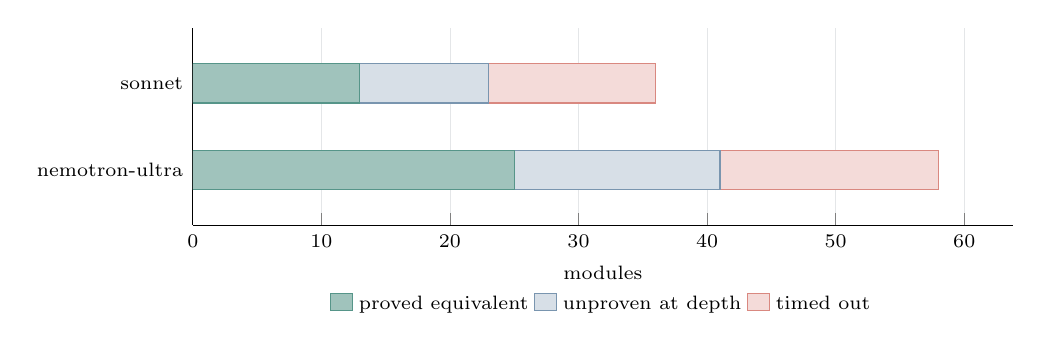
\begin{tikzpicture}
  \begin{axis}[
    xbar stacked, width=120mm, height=42mm,
    xmin=0,
    bar width=5mm, y=11mm, font=\scriptsize,
    xlabel={modules},
    ytick={0,1}, yticklabels={sonnet,nemotron-ultra},
    ytick style={draw=none}, y dir=reverse,
    axis x line*=bottom, axis y line*=left,
    xmajorgrids, grid style={rule!50, very thin},
    enlarge y limits={abs=7mm},
    legend style={at={(0.5,-0.3)}, anchor=north, draw=none,
                  legend columns=-1, font=\scriptsize},
    legend entries={proved equivalent, unproven at depth, timed out},
  ]
    \addplot[draw=accepted!80, fill=accepted!45] coordinates {(13,0) (25,1)};
    \addplot[draw=accent!60, fill=accent!18] coordinates {(10,0) (16,1)};
    \addplot[draw=critical!60, fill=critical!18] coordinates {(13,0) (17,1)};
  \end{axis}
  \end{tikzpicture}
  \end{adjustbox}
  \caption{Netlist-against-RTL equivalence per routed variant.}
  \label{fig:eqy}
  \par\smallskip\footnotesize\raggedright Neither of the two right-hand bands is a counterexample: no module in this run was shown inequivalent. They are the prover running out of depth or time, and they sit on the blocks whose timing is hard for the same reason.
\end{figure}


Of \eqychecked{} modules checked so far, \eqyproved{} are proved equivalent. The
remainder are unproven within the depth and time budget, not shown
inequivalent; no counterexample was found anywhere. They cluster on the deep
combinational blocks and the wide AXI interconnect, which is the difficulty
this project exists to attack: the blocks a prover struggles with
are the blocks whose timing does not close.

% =====================================================================
\section{Deliverable 7 --- Interactive demo}
\label{sec:d7}

\texttt{demo\_v2.py} walks the flow in eight acts, in the order it actually
runs: the sliced critical paths, the four arms over identical targets, the
gate funnel, the edits that survived, the clock audit and its runt-pulse
control, netlist equivalence, routed PPA, and finally a diff of the report's
own macros against the artifacts the demo just read. It is read-only: no API
key, no network, no toolchain. It finishes in about a second. A demo that
depends on a free-tier provider being up is a demo that fails in front of an
audience.

Act~3 is the part that demonstrates the gate rather than the generator: it
shows equivalent-but-wrong rewrites being caught and names the gate that caught
each one. For a live run, \texttt{bench/scripts/loop.py} takes the same targets
file and re-executes the whole loop against a backend of choice; the recorded
acts are that command's output from the runs this report is about.

% =====================================================================
\section{Model comparison}

\armstotal{} models ran in one invocation, over the same three targets, with
the same prompt, the same retry budget and the same gate configuration. Only
the backend changed, which is what makes the rows comparable. One row is still
not readable: an arm that lost calls to the harness defect
attempted fewer real edits than its proposal count suggests, so the count is
printed next to it rather than averaged away.

\begin{table}[htbp]
  \centering
  \footnotesize
  \caption{Four models over the same three targets, one invocation, identical gate configuration. Acceptance means every gate passed, not that the model produced plausible-looking RTL.}
  \label{tab:bakeoff}
  \begin{adjustbox}{max width=\textwidth}
  \begin{tabular}{lrrrrr}
    \toprule
    \textbf{Model} & \textbf{Proposals} & \textbf{Accepted} & \textbf{Cost (USD)} & \textbf{Harness losses} & \textbf{Wall (h)} \\
    \midrule
    gemini: gemini-flash & 3 & \textbf{0} & 0.01 & -- & 0.1 \\
    openrouter: nemotron-ultra & 21 & \textbf{1} & 0.00 & 0 of 4 & 3.1 \\
    anthropic: sonnet-direct & 13 & \textbf{1} & 2.65 & 7 of 8 & 0.5 \\
    anthropic: opus-direct & 13 & \textbf{0} & 13.51 & 8 of 9 & 0.6 \\
    \bottomrule
  \end{tabular}
  \end{adjustbox}
  \par\smallskip\footnotesize\raggedright \emph{Harness losses} are calls this harness threw away rather than the model declining: replies that exhausted the token budget inside reasoning and emitted no text. They are disclosed because an arm that lost calls attempted fewer real edits than its proposal count suggests, and comparing accept rates across arms without that is comparing two different experiments.
\end{table}


\begin{figure}[htbp]
  \centering
  \begin{adjustbox}{max width=\textwidth}
  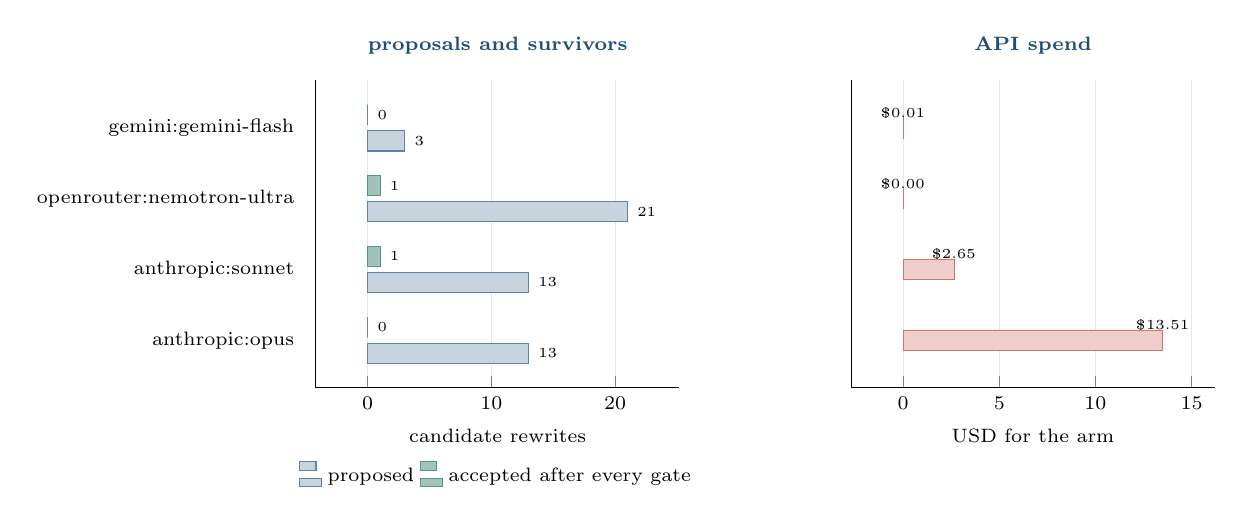
\begin{tikzpicture}
  \begin{axis}[
    title={proposals and survivors},
    title style={font=\scriptsize\bfseries, color=accent},
    xbar, width=62mm, height=52mm,
    bar width=2.6mm, y=9mm, font=\scriptsize,
    xlabel={candidate rewrites},
    ytick={0,1,2,3}, yticklabels={gemini:gemini-flash,openrouter:nemotron-ultra,anthropic:sonnet,anthropic:opus},
    ytick style={draw=none}, y dir=reverse,
    axis x line*=bottom, axis y line*=left,
    xmajorgrids, grid style={rule!50, very thin},
    enlarge y limits={abs=6mm}, enlarge x limits=0.2,
    nodes near coords, nodes near coords style={font=\tiny},
    legend style={at={(0.5,-0.22)}, anchor=north, draw=none, legend columns=-1, font=\scriptsize},
    legend entries={proposed, accepted after every gate},
  ]
    \addplot[xbar, draw=accent!70, fill=accent!25] coordinates {(3,0) (21,1) (13,2) (13,3)};
    \addplot[xbar, draw=accepted!80, fill=accepted!45] coordinates {(0,0) (1,1) (1,2) (0,3)};
  \end{axis}
  \begin{scope}[xshift=68mm]
  \begin{axis}[
    title={API spend},
    title style={font=\scriptsize\bfseries, color=accent},
    xbar, width=62mm, height=52mm,
    bar width=2.6mm, y=9mm, font=\scriptsize,
    xlabel={USD for the arm},
    ytick={0,1,2,3}, yticklabels={gemini:gemini-flash,openrouter:nemotron-ultra,anthropic:sonnet,anthropic:opus},
    ytick style={draw=none}, y dir=reverse,
    axis x line*=bottom, axis y line*=left,
    xmajorgrids, grid style={rule!50, very thin},
    enlarge y limits={abs=6mm}, enlarge x limits=0.2,
    nodes near coords, nodes near coords style={font=\tiny},
    yticklabels={,,}, ylabel={},
  ]
    \addplot[xbar, draw=critical!70, fill=critical!25, point meta=explicit symbolic] coordinates {(0.01,0) [\$0.01] (0.00,1) [\$0.00] (2.65,2) [\$2.65] (13.51,3) [\$13.51]};
  \end{axis}
  \end{scope}
  \end{tikzpicture}
  \end{adjustbox}
  \caption{Four models, one invocation, the same three targets and the same gates. Spend and survival are not related the way the price list suggests.}
  \label{fig:bakeoff}
  \par\smallskip\footnotesize\raggedright Same run as Table~\ref{tab:bakeoff}. The accepted bar counts rewrites that passed every gate, not replies that looked like Verilog.
\end{figure}


\subsection{What survived}

\armssurviving{} of \armstotal{} arms produced a rewrite that passed every
gate, and the two that did converged: the same module, the same transform
class, found independently. One of them cost \$\armcheapcost{}
(\armcheapname, on a free endpoint) and took \armcheaphours\,h. The other
cost \$\armpaidcost{} (\armpaidname) and took \armpaidhours\,h. The difference on this workload is therefore about six times the wall clock
against about three dollars. The routed results do not distinguish the two:
the netlists agree to within \bestagreement\,ns.

\subsection{What the spend did not buy}

\armtopname{} was the most expensive arm at \$\armtopcost{} and finished with
\armtopaccepted{} accepted rewrites. We do not read that as a ranking. Of its
\armtopproposals{} calls, \armtoplost{} returned no usable text at all, which
is this harness truncating a reply mid-reasoning rather than the model
declining, and the defect was fixed after these runs. This arm spent the most and
produced the fewest usable proposals, but the run was not a fair test of it, so
no conclusion about the model is drawn from it.

\subsection{Where each arm's candidates died}

\begin{table}[htbp]
  \centering
  \footnotesize
  \caption{Where each arm's candidates stopped. Same four arms, same targets, same gate configuration as Table~\ref{tab:bakeoff}.}
  \label{tab:deaths}
  \begin{adjustbox}{max width=\textwidth}
  \begin{tabular}{lrrrrrr}
    \toprule
    \textbf{Model} & \textbf{propose} & \textbf{validate} & \textbf{g1} & \textbf{g1b} & \textbf{accepted} & \textbf{backend} \\
    \midrule
    gemini:gemini-flash & -- & -- & 1 & -- & -- & 1 \\
    openrouter:nemotron-ultra & 4 & 10 & 4 & 1 & \textbf{1} & -- \\
    anthropic:sonnet & 8 & -- & 2 & 1 & \textbf{1} & -- \\
    anthropic:opus & 9 & -- & 2 & 1 & -- & -- \\
    \bottomrule
  \end{tabular}
  \end{adjustbox}
  \par\smallskip\footnotesize\raggedright \texttt{propose} counts calls that returned no usable text, which on three of these arms is the harness defect rather than the model refusing. \texttt{validate} counts proposals rejected before any prover ran, for changing an interface or leaving the permitted transform set. \texttt{g1} is a failed or unfinished equivalence proof and \texttt{g1b} a proof that succeeded at the module and failed at its parent.
\end{table}


Table~\ref{tab:deaths} breaks the losses down by gate. The arms fail at
different stages, and the corresponding fixes are different. \armcheapname{} reached the gates most often and lost
most of its candidates at \texttt{validate}, before a prover was ever started,
by proposing edits outside the permitted transform set or by changing an
interface it was told to leave alone; that is a prompt and parser problem. The
two Anthropic arms lost their candidates earlier, inside the call itself, which
was the harness defect above. \texttt{gemini-flash} ran for
minutes, proposed three times, and returned nothing the gates could act on.

One column is the same for every arm that reached it. The three arms that ever
cleared \texttt{g1} each then lost a candidate at \texttt{g1b}, the
parent-contract gate: a rewrite proved equivalent to the module it replaced and
still wrong in the design. Three models from three vendors produced the same
defect, which is the main evidence for checking it mechanically rather than by
review.

% =====================================================================
\section{Thought process}
\label{sec:journey}

Most of the structural decisions in this system came from runs that reported a
result we later found to be wrong. Those are the expensive failures here: a
crash is caught immediately, while a flow that reports closure it did not
achieve is not. The subsections below are in the order the problems appeared.

\subsection{The benchmark had bugs before any model saw it}

The first benchmark we wrote passed synthesis, passed simulation, and had two
defects in its clock structures: an enable that reached a clock gate without
being retimed onto the inactive edge, and a divider output selected by a
combinational mux. Both produce runt pulses --- a clock edge too narrow to be a
clock edge --- and neither shows up in a slack number. We found them by
writing the audit that is now the G1c/G2c gate, and we fixed them in the
benchmark rather than tuning the audit until the benchmark passed. The control
in Figure~\ref{fig:runt} is that audit run against the broken version.

Two rules follow from this and are applied throughout: the input RTL is frozen
only after it has been audited, and no gate is used in the flow until it has
been shown rejecting a known-bad case.

\subsection{The slicer was reading the wrong netlist}

The first loop runs stopped with nothing to do: the slicer was reading the
post-resizer netlist, and the resizer had already hidden two of the three
violating domains in buffering (Section~\ref{sec:d1}). Every target list in
this report is sliced from the post-synthesis database instead.

\subsection{Most of the call budget was spent on paths no rewrite can reach}

Early runs spent the majority of their API calls on targets where the critical
path sits in a macro, a clock network, or an I/O constraint --- places none of
the four permitted transforms can touch. The model returned a
plausible rewrite of the nearest module and the gates rejected it. Targets
now carry a lever annotation: no lever, no call, still reported and still
counted as a violation. The same budget then buys proposals against paths a
rewrite can actually move.

\subsection{A proposal that changed nothing was counted as a closed path}

One arm re-proposed an already-accepted edit under a second module's name and
the loop counted a second closed path. That run is what put the scope rule in
Section~\ref{sec:scope} into the flow.

\subsection{Pipelining forced the parent into the proof}

The first pipelining proposals were rejected outright, which is what the
\texttt{submodules} channel in Section~\ref{sec:multimodule} was built for.
Making those edits reachable produced the next failure directly: rewrites proved
equivalent at the module and wrong at the parent, which is where G1b came from.

\subsection{The biggest loss in the funnel was ours}

Reading the first funnel showed the largest single cause of rejection was our
own truncation defect rather than a gate (Section~\ref{sec:d3}). It hit the
reasoning-heavy arms hardest, which biases the bake-off towards the cheaper
models, so the affected arms are marked in every table built from those runs
instead of the rows being removed.

\subsection{Global WNS was not a usable metric on this design}

The first routed comparison was read off global WNS, which moved in the wrong
direction while two domains improved. Following that showed global WNS here is
set by the divider path and moves further between two placements of the same
netlist than under any accepted edit, which is why Section~\ref{sec:d5} reports
per domain. The second routed generation was run to see whether the surviving
claim reproduced on an independent floorplan with its own baseline.

% =====================================================================
\section{Innovation}
\label{sec:innovation}

Five features of this system are absent from the published work compared
against in Section~\ref{sec:related}. Each was added after a run failed without
it, and each has a measurement in this report behind it.

\begin{enumerate}[leftmargin=1.4em]
  \item \textbf{Equivalence gate with a recorded proof depth.} An edit enters
        the optimised RTL only with an EQY result attached, and the depth of
        that result is stored with it. A combinational rewrite is proved
        complete in one miter cycle, a feed-forward pipeline insertion at
        latency${}+2$, and every other case is bounded with its bound printed
        beside the result rather than folded into a pass count
        (Section~\ref{sec:gates}). A flow that accepts on simulation does not
        separate those cases.

  \item \textbf{A separate gate for the parent's timing contract (G1b).}
        \numcontractkills{} rewrites passed G1 with a complete proof and were
        rejected by G1b at the parent (Table~\ref{tab:g1b}), and they came from
        three different models. This is the report's main result.

  \item \textbf{Multi-module proposals, so latency-changing edits are
        reachable.} Pipelining changes latency, and a single-module
        equivalence check rejects any latency change. A proposal therefore
        carries a \texttt{submodules} field: it rewrites the target and every
        parent that must wait for it, and the set is proved together
        (Section~\ref{sec:multimodule}). Without that field, pipelining is
        unreachable.

  \item \textbf{Accepted scope taken from the working-tree diff.} The loop
        computes what an edit changed by diffing the tree, not by reading the
        module list in the proposal. A proposal whose diff is empty is
        recorded as a no-op rather than a closed path
        (Section~\ref{sec:scope}). Without this, one accepted edit re-sent
        under a second module's name is counted twice and the headline number
        rises with no work behind it.

  \item \textbf{Slack reported per clock domain, with the noise floor
        stated.} The design has five mutually asynchronous masters, so a
        single global WNS mixes five independent questions. Global WNS here is
        set by a divider path that no permitted transform reaches, and it
        moves further between two placements of the same netlist than under
        any accepted edit. The headline claim is therefore restricted to the
        domain where two structurally different rewrites agree to within
        \bestagreement\,ns; domains where the two disagree in sign are
        reported as placement noise.
\end{enumerate}

% =====================================================================
\section{What this does not claim}

\begin{itemize}
  \item The \baselinewns\,ns divider path did not close. No transform in the
        permitted set reaches it without a latency change, and the parent
        handshake that a latency change requires is the open problem.
  \item Gains are per-domain. Chip frequency is still governed by the slowest
        domain, and that domain is the one above.
  \item Modules that time out in the netlist check are unproven, not proved.
        We report the distinction rather than the aggregate.
  \item The clock structures were repaired after the audit found them, and
        the repair is backed by a runt-pulse simulation
        (Table~\ref{tab:clockrisk}), not by the structural auditor alone. The
        auditor matches known unsafe shapes and cannot detect one it has no
        rule for, so G2c is a regression gate, not a clock-quality
        certificate.
  \item CDC gates assume Gray or handshake encoding on multi-bit crossings
        rather than proving it. The assumption is recorded in every run's
        warnings, including the baseline's.
\end{itemize}

% =====================================================================
\appendix
\section{The accepted rewrite, in full}

Table~\ref{tab:accepts} says an edit to \texttt{fp8\_adder} was accepted and
proved. This is that edit, cut out of \texttt{diff -u} at build time rather
than transcribed, so it cannot drift from the RTL that was actually measured.

Both models found the same target, a nine-iteration sequential leading-one
search written as a \texttt{for} loop that synthesises to nine serial compares,
and both replaced it with a single-level parallel priority match. The two
implementations differ in size by an order of magnitude: one changed
\difflinessonnet{} lines, the other \difflinesnemotronultra{}. The routed
results still land within \bestagreement\,ns of each other, which is why the
improvement is attributed to the transform rather than to either model.

\paragraph{sonnet.} 38 changed lines in total; the hunk that carries the transform:
\begin{lstlisting}[style=diff]
@@ -185,17 +175,25 @@
                 sing_reg = b[7];
         end
 
-       /////// leading  one detector 
-       
+       /////// leading  one detector -- rewritten as a balanced priority casez
+       /////// instead of a 9-iteration sequential for loop. Same priority
+       /////// order (highest set bit wins), same result every cycle, but
+       /////// the dependency chain collapses from 9 serial compares to a
+       /////// single-level parallel priority match.
 
-        for (i = 8; i >= 0; i = i - 1)
-        begin
-            if ((sum_mant[i] == 1'b1) && (found == 1'b0))
-            begin
-                leading_1_index = i[4:0];
-                found = 1'b1;
-            end
-        end
+        casez (sum_mant[8:0])
+            9'b1????????: leading_1_index = 5'd8;
+            9'b01???????: leading_1_index = 5'd7;
+            9'b001??????: leading_1_index = 5'd6;
+            9'b0001?????: leading_1_index = 5'd5;
+            9'b00001????: leading_1_index = 5'd4;
+            9'b000001???: leading_1_index = 5'd3;
+            9'b0000001??: leading_1_index = 5'd2;
+            9'b00000001?: leading_1_index = 5'd1;
+            9'b000000001: leading_1_index = 5'd0;
+            default:      leading_1_index = 5'd0;
+        endcase
+        found = |sum_mant[8:0];
 
 
\end{lstlisting}
\paragraph{nemotron-ultra.} 299 changed lines in total; the hunk that carries the transform:
\begin{lstlisting}[style=diff]
@@ -46,249 +46,132 @@
@@ ... 126 lines earlier in the same hunk ...
+        mant_a_reg = b_grater_reg ? {2'b00, (({mant_a, 4'd0}) >> shift_b) | {7'b0, sticky_a}} : {2'b00, {mant_a, 4'd0}};
+        mant_b_reg = a_grater_reg ? {2'b00, (({mant_b, 4'd0}) >> shift_a) | {7'b0, sticky_b}} : {2'b00, {mant_b, 4'd0}};
 
+        // Complement for subtraction
+        a_operand = ((b[6:0] > a[6:0]) && (a[7] ^ b[7])) ? ~mant_a_reg : mant_a_reg;
+        b_operand = ((a[6:0] > b[6:0]) && (a[7] ^ b[7])) ? ~mant_b_reg : mant_b_reg;
+        sum_mant  = a_operand + b_operand + {10'b0, (a[7] ^ b[7])};
 
-        if (shift_b == 4'd0)
-            sticky_a = 1'b0;
-        else if (shift_b >= 4'd8)
-            sticky_a = |{mant_a,4'd0};
-        else
-            sticky_a = |(({mant_a,4'd0}) & (8'hFF >> (8 - shift_b)));
+        // Sign
+        sing_reg = (a[7] == b[7]) ? a[7] : (a[6:0] >= b[6:0] ? a[7] : b[7]);
 
-        if (shift_a == 4'd0)
-            sticky_b = 1'b0;
-        else if (shift_a >= 4'd8)
-            sticky_b = |{mant_b,4'd0};
-        else
-            sticky_b = |(({mant_b,4'd0}) & (8'hFF >> (8 - shift_a)));
-            
-            
+        // Leading-one detector: parallel casez instead of for-loop priority chain
+        casez (sum_mant[8:0])
+            9'b1????????: leading_1_index = 5'd8;
+            9'b01???????: leading_1_index = 5'd7;
+            9'b001??????: leading_1_index = 5'd6;
+            9'b0001?????: leading_1_index = 5'd5;
+            9'b00001????: leading_1_index = 5'd4;
+            9'b000001???: leading_1_index = 5'd3;
+            9'b0000001??: leading_1_index = 5'd2;
\end{lstlisting}
\paragraph{sonnet\_wide.} 183 changed lines in total; the hunk that carries the transform:
\begin{lstlisting}[style=diff]
@@ -185,20 +207,27 @@
                 sing_reg = b[7];
         end
 
-       /////// leading  one detector 
-       
+       /////// leading one detector (flat casez priority encoder)
 
-        for (i = 8; i >= 0; i = i - 1)
-        begin
-            if ((sum_mant[i] == 1'b1) && (found == 1'b0))
-            begin
-                leading_1_index = i[4:0];
-                found = 1'b1;
-            end
-        end
+        casez (sum_mant[8:0])
+            9'b1????????: begin leading_1_index = 5'd8; found = 1'b1; end
+            9'b01???????: begin leading_1_index = 5'd7; found = 1'b1; end
+            9'b001??????: begin leading_1_index = 5'd6; found = 1'b1; end
+            9'b0001?????: begin leading_1_index = 5'd5; found = 1'b1; end
+            9'b00001????: begin leading_1_index = 5'd4; found = 1'b1; end
+            9'b000001???: begin leading_1_index = 5'd3; found = 1'b1; end
+            9'b0000001??: begin leading_1_index = 5'd2; found = 1'b1; end
+            9'b00000001?: begin leading_1_index = 5'd1; found = 1'b1; end
+            9'b000000001: begin leading_1_index = 5'd0; found = 1'b1; end
+            default:      begin leading_1_index = 5'd0; found = 1'b0; end
+        endcase
 
 
-     //////// normilization 
+     //////// normalization -- candidates for every branch computed
+     //////// unconditionally in parallel; the branch conditions only pick
+     //////// among finished values (single flat mux level) instead of the
+     //////// original 3-deep nested if/else forcing each candidate's
\end{lstlisting}


\section{The contract the model is held to}

This is the system prompt, quoted out of \texttt{bench/scripts/loop.py} at
build time. Almost every constraint in it was added because a run failed
without it: the reset rule exists because a pipeline stage given a reset the
original module did not have disagrees with its own unpipelined self while
reset is asserted, and the equivalence checker correctly reports that as a
counterexample. The rule against replacing structural arithmetic with a
behavioural operator exists because three such answers cost \SI{2400}{\second}
each and returned no verdict at all. Rewriting a restoring divider as
\texttt{a / b} does not shorten the path; it hands the prover a hard arithmetic
theorem.

The diagnosis fields are read directly into this report, so the prompt requires
them to describe the path in front of the model rather than give general
timing-closure advice.

\begin{lstlisting}[style=plain]
You optimise Verilog RTL to close timing. You are given one
critical path from a placed and routed design, the RTL module that owns most
of its delay, and a catalogue of transforms you may apply.

Reply with a single JSON object and nothing else:

  {"transform": "<catalogue name>",
   "module": "<module you are rewriting>",
   "latency_delta": <integer cycles the module's outputs are delayed by>,
   "rtl": "<the complete rewritten module, module...endmodule>",
   "submodules": {"<child module name>": "<its complete rewritten source>"},
   "which_path": "<the failing path in one sentence: what it runs from, what
                  it runs to, and which module or instances own the delay>",
   "why": {"cause": "<exactly one of: logic_depth, high_fanout, clock_skew,
                     net_delay, congestion, low_drive_strength, other>",
           "evidence": "<the numbers above that support that cause>"},
   "what": {"rtl_level_fix": "<the transform you are applying, and why it
                              shortens this path>",
            "tool_level_fix": "<what synthesis or place-and-route could do
                               about this path instead, or \"none\" if the
                               tools cannot reach it>"}}

`submodules` is optional and usually absent. Include it only when the
transform genuinely spans two levels -- pipelining a combinational child, for
example, puts the stage registers inside the child and the control that tracks
them in the parent, and neither half is correct on its own. A child listed
there may change its own port list, because parent and child are replaced
together. A child that anything OUTSIDE this proposal instantiates may not be
listed at all; that is checked and will reject your answer.

Rules that are checked mechanically and will reject your answer:
  - `rtl` must define exactly the module named in `module`, with an identical
    port list: same names, same directions, same widths. This applies to the
    target module only; a module listed in `submodules` may change its ports.
  - `latency_delta` must be 0 for a latency-preserving transform, and the
    exact number of cycles added for a latency-changing one. A wrong value is
    a rejection, not a rounding error.
  - You may not edit a module that carries a clock-domain crossing.
  - Preserve the module's existing reset behaviour. In particular, a register
    you ADD to a feed-forward datapath must not be given a reset the original
    module did not have. Such a register holds no state that has to be
    recovered, a reset on it is wasted area, and it makes the module disagree
    with its own unpipelined self for as long as reset is asserted -- which
    the equivalence check reports as a counterexample. Write the new stage as
    a bare `always @(posedge clk) q <= d;` with no reset branch.
  - Do not replace an explicit structural arithmetic block with a behavioural
    operator. Rewriting a 32-step restoring divider as `a / b`, or an array
    multiplier as `a * b`, does not shorten the path: synthesis expands the
    operator back into a comparable structure, so the same logic depth comes
    back under a different name. It also hands the equivalence checker the
    task of proving a hand-written division algorithm equal to the `/`
    operator, which is a hard arithmetic theorem and not the question anyone
    asked -- three such answers cost 2400 seconds each and returned no verdict
    at all. If an arithmetic block is the bottleneck, pipeline it, retime it
    or restructure it INTO stages; do not delete its structure.

`which_path`, `why` and `what` are the diagnosis, not decoration. They are
read straight into the report, so write them about THIS path with the numbers
from the timing data above, not as general advice about timing closure.

`what.tool_level_fix` is asked for even though you are not applying it, and
answering it honestly matters: most of these paths are already past what the
tools can do -- the design has been through resizing and buffering before you
see it -- and saying so is the argument for why an RTL edit was needed at all.
Write "none" and say why, rather than inventing a tool fix that would not
work.

SCOPE. `module` is the module you are rewriting and it must be the TARGET
module named in the prompt, not one of the modules it instantiates. If the fix
needs a child rewritten too, put the child in `submodules` and keep the target
in `module`. Rewriting a child alone, with the child's name in `module`, is
rejected without being read: the loop can only splice an edit it asked for.

LATENCY. An edit that adds a pipeline stage changes when the target's outputs
arrive, and every parent that consumes them in the same cycle it drives the
inputs then breaks. On this design that has rejected four proposals. So a
latency change is only worth proposing as ONE proposal that rewrites the
target AND, through `submodules`, every parent that has to learn to wait --
a valid/ready or stall handshake, written out, not assumed. A deep
combinational block whose only fix is multi-cycle is exactly this case: it is
allowed, it is not a new module, and it is the one way such a path closes.

If no catalogue transform helps this path, reply {"refused": "<why>"}.
\end{lstlisting}


\end{document}
